%% LaTeX2e class for student theses
%% thesis.tex
%% 
%% Karlsruhe Institute of Technology
%% Institute for Program Structures and Data Organization
%% Chair for Software Design and Quality (SDQ)
%%
%% Dr.-Ing. Erik Burger
%% burger@kit.edu
%%
%% Version 1.3.2, 2017-08-01

%% Available page modes: oneside, twoside
%% Available languages: english, ngerman
%% Available modes: draft, final (see README)

\documentclass[twoside, english]{sdqthesis}

\usepackage[T1]{fontenc}
\usepackage{lmodern}

\usepackage{listings}             % Include the listings-package
\definecolor{javared}{rgb}{0.6,0,0} % for strings
\definecolor{javagreen}{rgb}{0.25,0.5,0.35} % comments
\definecolor{javapurple}{rgb}{0.5,0,0.35} % keywords
\definecolor{javadocblue}{rgb}{0.25,0.35,0.75} % javadoc
 
\lstset{language=Java,
basicstyle=\ttfamily,
keywordstyle=\color{javapurple}\bfseries,
stringstyle=\color{javared},
commentstyle=\color{javagreen},
morecomment=[s][\color{javadocblue}]{/**}{*/},
numbers=left,
numberstyle=\tiny\color{black},
stepnumber=1,
numbersep=6pt,
tabsize=1,
breaklines=true,
showspaces=false,
showstringspaces=false}


%% ---------------------------------
%% | Information about the thesis  |
%% ---------------------------------

%% Name of the author
\author{Noureddine Dahmane}

%% Title (and possibly subtitle) of the thesis
\title{Adaptive Monitoring for Continuous Performance Model Integration}

%% Type of the thesis 
\thesistype{Master’s Thesis}

%% Change the institute here, ``IPD'' is default
% \myinstitute{Institute for \dots}

%% You can put a logo in the ``logos'' directory and include it here
%% instead of the SDQ logo
% \grouplogo{myfile}
%% Alternatively, you can disable the group logo
 \nogrouplogo

%% The reviewers are the professors that grade your thesis
\reviewerone{Prof. Anne Koziolek}

\reviewertwo{Prof. Ralf Reussner}

%% The advisors are PhDs or Postdocs
\advisorone{M.Sc. Manar Mazkatli}


%% Please enter the start end end time of your thesis
\editingtime{01. August 2018}{14. March 2019}

\settitle

%% --------------------------------
%% | Settings for word separation |
%% --------------------------------

%% Describe separation hints here.
%% For more details, see 
%% http://en.wikibooks.org/wiki/LaTeX/Text_Formatting#Hyphenation
\hyphenation{
% me-ta-mo-del
}

%% --------------------------------
%% | Bibliography                 |
%% --------------------------------

%% Use biber instead of BibTeX, see README
\usepackage[citestyle=numeric,style=numeric,backend=biber]{biblatex}
\addbibresource{thesis.bib}



%% ====================================
%% ====================================
%% ||                                ||
%% || Beginning of the main document ||
%% ||                                ||
%% ====================================
%% ====================================
\begin{document}

%% Set PDF metadata
\setpdf

%% Set the title
\maketitle

%% The Preamble begins here
\frontmatter

%% LaTeX2e class for student theses: Declaration of independent work
%% sections/declaration.tex
%% 
%% Karlsruhe Institute of Technology
%% Institute for Program Structures and Data Organization
%% Chair for Software Design and Quality (SDQ)
%%
%% Dr.-Ing. Erik Burger
%% burger@kit.edu
%%
%% Version 1.3.2, 2017-08-01

\thispagestyle{empty}
\null\vfill
\noindent\hbox to \textwidth{\hrulefill} 
\iflanguage{english}{I declare that I have developed and written the enclosed
thesis completely by myself, and have not used sources or means without
declaration in the text.}%
{Ich versichere wahrheitsgemäß, die Arbeit
selbstständig angefertigt, alle benutzten Hilfsmittel vollständig und genau
angegeben und alles kenntlich gemacht zu haben, was aus Arbeiten anderer
unverändert oder mit Änderungen entnommen wurde.}
 
 
%% ---------------------------------------------
%% | Replace PLACE and DATE with actual values |
%% ---------------------------------------------
\textbf{PLACE, DATE}
\vspace{1.5cm}
 
\dotfill\hspace*{8.0cm}\\
\hspace*{2cm}(\theauthor) 


\setcounter{page}{1}
\pagenumbering{roman}

%% ----------------
%% |   Abstract   |
%% ----------------
 
%% For theses written in English, an abstract both in English
%% and German is mandatory.
%%
%% For theses written in German, a German abstract is sufficient.
%%
%% The text is included from the following files:
%% - sections/abstract



%% ------------------------
%% |   Table of Contents  |
%% ------------------------
\tableofcontents

\listoffigures

%% -----------------
%% |   Main part   |
%% -----------------

\mainmatter
%% LaTeX2e class for student theses
%% sections/abstract_en.tex
%% 
%% Karlsruhe Institute of Technology
%% Institute for Program Structures and Data Organization
%% Chair for Software Design and Quality (SDQ)
%%
%% Dr.-Ing. Erik Burger
%% burger@kit.edu
%%
%% Version 1.3.2, 2017-08-01

\Abstract
Model-driven performance prediction can be used in order to predict software performance at the design stage. Applying it in the agile development process can reduce time and effort spent on monitoring. However, building such a model manually is impractical in the agile development process because it tends to generate quick releases in shot cycles. Existing approaches that extract automatically Performance Model (PM) are based on reverse-engineering and/or measurement techniques. However, these approaches require to monitor and analyze the whole system after each iteration, which will cause a monitoring overhead. 

The approaches that extract incrementally the PM from the source code and keep them consistent need a monitoring approach that provide them with the required monitoring information. Existing approaches either cannot provide fine-grained monitoring information or the instrumentation of the source code has to be done manually which is unsuitable for developers.

To overcome these problems, this thesis introduces an approach that can monitor the system in an adaptive way and provide PMs with the fine-grained monitoring information. Moreover, our approach is part of the continuous integration of PMs in the agile development process. We achieved this by introducing an automatic adaptive instrumentation approach of the source code. Furthermore, our instrumentation approach can monitor changes in the source code during system development and instrument the changed parts of the source code accordingly and automatically. During the system development, we collect automatically the monitoring probes that are needed to instrument the source code. When changes in the source code are committed, we automatically instrument the source code based on the monitoring probes that we've generated during the system development. The benefit of our approach will be to reduce the high monitoring overhead and to support the continuous integration of performance models.  

In particular, our approach can be integrated with other approaches that keep the source code and the PM consistent. While these approaches tend to keep the source code and its behavior in terms of PM consistent, our approach will provide them with the needed monitoring data to estimate the PM parameters (like Resource Demands RDs, loop execution number, the probability of selecting a branch).  

We evaluated our approach based on a case study. we showed that we could instrument incrementally and automatically the source code. Moreover, our evaluation showed that we could provide monitoring information that can be used for the calibration of performance model parameters considering parametric dependencies. Furthermore, using our approach and the case study we showed that we could reduce the monitoring overhead to 50\%. 
%% LaTeX2e class for student theses
%% sections/content.tex
%% 
%% Karlsruhe Institute of Technology
%% Institute for Program Structures and Data Organization
%% Chair for Software Design and Quality (SDQ)
%%
%% Dr.-Ing. Erik Burger
%% burger@kit.edu
%%
%% Version 1.3.2, 2017-08-01

\chapter{Introduction}
\label{ch:Introduction}

%% -------------------
%% | Example content |
%% -------------------

Software performance is a quality attribute, which determines whether a given system has the ability to perform the functional requirements in terms of acceptable scalability and responsiveness. Many applications crash or cannot be applied because the performance problems have been not taken into account during development. 

In order to avoid performance issues, performance aspects must be captured and treated during system development. Performance tests can be used to decide if the system meets its requirements. However, using it in a huge application can be too expensive because we need to allocate resources and generate measurements of an application, which creates a massive load. 

Performance tests can be altered by performance model prediction, which can reduce the costs of performance tests. A performance model represents an abstraction of the behavior as well as the performance-relevant aspects of the system. Moreover, performance model prediction solves performance problems by using performance models and simulation engines. Performance simulation requires only a fraction of resources to evaluate the performance of a system. Another advantage of model-based performance prediction is the capability of identifying performance issues before implementation, which then helps to correct design problems as early as possible. 

Model-based performance prediction can be used in the modern agile development process to support design decisions and reduce the costs of measurement-based performance evaluation. However, Existing approaches have two shortcomings. (1) they do not extract incrementally the performance model, which means if they will be used iteratively, they will extract the performance model of the whole system in each iteration. This can guide to a high monitoring overhead in case of huge systems. Moreover, extracting the performance model in such way will not keep the old modifications of the performance in each iteration.  (2) the existing techniques do not come up with performance model parameters (like Resource Demands, loop execution number, the probability of selecting a branch) and their dependencies with impacting factors like input data.

There exist approaches that extract incrementally the performance model from the source code and keep them consistent. For example, Langhammer introduced an approach \cite{langhammer2017automated} that keep the source code and architecture consistent include the performance model in term of Service Effect Specification (SEFF) \ref{sec: SEFFs}. Furthermore, Mazkatli and Koziolek have extended his approach by introducing an approach that uses the Continuous Integration (CI) and Continuous Deployment of the source code and extend them with the Continuous Integration of a Performance Model (CIMP) \cite{mazkatli2018continuous}. Both presented approaches require an adaptive monitoring approach that provides them with the required monitoring information and can be integrated into the continuous integration of the performance model. 

In this thesis, we present an approach for adaptive monitoring for continuous performance model integration. Our approach can be used incrementally to provide monitoring information for continuous performance model integration. In particular, we used the performance model of the Palladio Component Model (PCM)(Section \ref{sec:The Palladio Component Model}), which describes the behavior and the performance aspects of the system in term of SEFF. Furthermore, our approach can provide the monitoring information that can be used to estimate the SEFF model parameters. We provide monitoring information of computation response time, loop execution number, the probability of selecting a branch and the parameters of service calls, which can be used to consider the parametric dependencies in SEFF model parameters estimation.

In order to achieve incremental instrumentation of the source code, our approach uses the change-driven framework Vitruvius (Section \ref{sec:Vitruvius}) and we extended the Coevolution approach \cite{langhammer2017automated} of Langhammer. Vitruvius provides the possibility to keep model instances consistent via consistency preservation rules can be defined by the user. Moreover, Langhammer used Vitruvius to generate incrementally SEFF models, but he did not provide an adaptive monitoring approach to provide SEFF Models with the required monitoring information. Moreover, we contributed to Vitruvius by presenting an Instrumentation Model (IM) (Section \ref{sec:Adaptive Instrumentation}), which describes the instrumentation points, which are needed for the source code instrumentation. Then, we defined the consistency preservation rules that keep the source code model and IM consistent. Using Vitruvius, we could in each iteration capture changes in the source code and create accordingly the instrumentation points. Therefore, we could instrument the source code incrementally. 

Our approach is part of the vision presented by Mazkatli and Koziolek \cite{mazkatli2018continuous}. They extended the agile development process by introducing an approach that automatically and continuously integrates the performance model. 

In chapter \ref{ch:Foundations} we explain the foundation of our approach. In chapter \ref{ch:Thesis Statement} we define our contributions. In chapter \ref{ch:Adaptive Monitoring for Continuous Performance Model Integration} we describe our approach. In chapter \ref{ch:Evaluation} we a case study to evaluate out approach. In chapter \ref{ch:Related Work} we discuss the related work. Chapter \ref{ch:Conclusions and Future Work} gives a summary of this thesis and feature work. 


%% LaTeX2e class for student theses
%% sections/content.tex
%% 
%% Karlsruhe Institute of Technology
%% Institute for Program Structures and Data Organization
%% Chair for Software Design and Quality (SDQ)
%%
%% Dr.-Ing. Erik Burger
%% burger@kit.edu
%%
%% Version 1.3.2, 2017-08-01


\chapter{Foundations}
\label{ch:Foundations}
In this section, we introduce the necessary foundations for this thesis. In section \ref{sec:The Palladio Component Model}, we present the Palladio Component Model (PCM) and it's models. In section \ref{sec: SEFFs}, we describe briefly the Service Effect Specification (SEFF) model of PCM. In section \ref{sec:Vitruvius}, we present the Vitruvius Framework. In section \ref{sec:Java Model Parser and printer}, we present Java Model Parser and Printer (JaMoPP). In section \ref{sec:Automated Coevolution of Source Code and Software Architecture Models}, we introduce the Coevolution approach \cite{langhammer2015co}. In section \ref{sec:Kieker Monitoring}, we present the Kieker Monitoring Framework. In section \ref{sec:Source Code Model eXtractor}, we give an overview of the reverse-engineering of the approach Source Code Model eXtractor (SoMoX). In section \ref{sec:Continuous Integration of Performance Model}, we bring in the approach Continuous Integration of Performance Model (CIPM). In section \ref{sec:Iterative Performance Model Parameter Estimation Considering Parametric Dependencies}, we summarize the master thesis of Jägers. In the last section \ref{sec:DevOps}, we introduce the development process DevOps.

\section{Eclipse Modeling Framework}
\label{sec:Eclipse Modeling Framework}
Eclipse Modeling Framework (EMF) is a framework, that enable the creation of meta-models based on Ecore. Moreover, EMF provides the following facilities:
\begin{itemize}
\item Source code generation from meta-models. 
\item Generate an instance of eclipse in order to instantiate meta-models and edit them.
\end{itemize}    

\section{The Palladio Component Model}
\label{sec:The Palladio Component Model}
Palladio Component Model (PCM) is a component-based software architecture approach, that can be used to predict and evaluate the performance and the reliability of component-based software systems at design stage. For performance prediction, it makes it possible to analyze the components of the software architectures before implementation and thus it can for example detects bottlenecks, predict response time and predict throughput. For software reliability, PCM specifies metrics like detecting the probability of failures on demand. 

\subsection{Palladio Models}
\label{sec: Palladio Models}
To allow the prediction of the Performance and the reliability of a software system, PCM defines four different roles to create four different models \ref{fig:PCM Models and transformations}. The Repository model, which is created by developers. Developers specify and implement components, interfaces, provided roles, required roles and signatures for the repository. In the context of PCM, a component is by definition a block of software, that can be composed, deployed and customized without requiring the understanding of its internals.  Moreover, the roles in PCM specify the relation between the components and the interfaces. Developers should also specify the internal behavior of the components in term of Service Effect Specification (SEFF). The Assembly model is created by software architects. Software architects use the existing components in repository to create the software system. The allocation model is created by system deployers.  Deployers are responsible for specifying the environment resource, like Servers, CPUs, HDDs and network connection. Afterwards, they decide which assembly can be deployed in which resource. The usage model is created by domain experts. Domain experts provide information about the interaction between the system and the users. Additionally, domain experts can define the relevant critical usage scenarios and the inputs parameters values. 

In the context of this thesis, we will use the information provided by SEFFs. Thus, we will explore the related concepts based on \cite{becker2009palladio} and \cite{koziolek2006parameter}.

\begin{figure}[h]
\centering
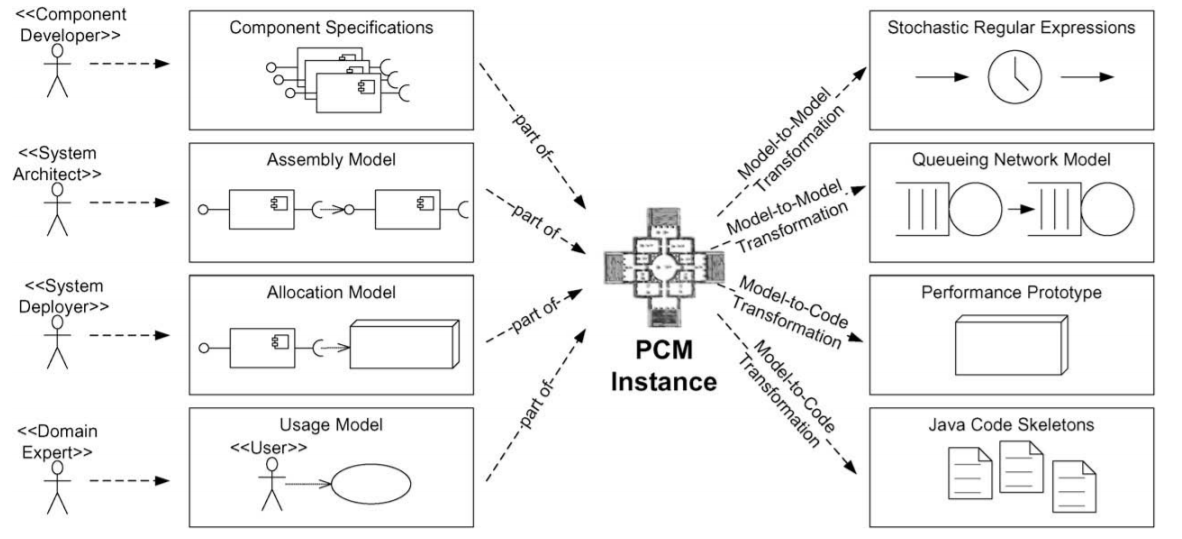
\includegraphics[width=0.9\textwidth]{figures/pcmmodels}
\caption{PCM Models and transformations \cite{reussner2016modeling}}
\label{fig:PCM Models and transformations}
\end{figure}


\subsection{SEFFs}
\label{sec: SEFFs}
Service Effect Specification (SEFF) were firstly presented by \cite{koziolek2006parameter}, which describes like a UML Activity Diagram the control flow of component services. For each provided service, SEFF describes how services in the required interface are called in the provided service. Moreover, as mentioned before, the components in PCM can be used without understanding their internals and thus as a black box. However, SEFF turns a component to a gray box by describing the behavior of its provided services.
The ResourceDemandingServiceEffectSpecifaction (RDSEFF) used in PCM to predict the performance, is an extension of SEFF. RDSEFF offers the possibility to add performance inputs values associated to each activity of SEFF. Moreover, to each component provided service, developers can specify a RDSEFF in order to describe how the service uses the hardware/software resources and how it calls the component's required services. 
In the rest of this thesis, we will indicate RDSEFF as SEFF in order to avoid ambiguity. The principal elements of SEFF will be explored in the following. SEFF includes the so called ExternalCallActions which present the call of a required Service within the SEFF. InternalActions are used within SEFF to abstract the internal computation of the component. Moreover, an internal action can be defined as a set of successive instruction, that do not include any external call from other components. LoopActions within SEFF are specified to indicate the number of times the sub control flow within the loop is going to be executed. BranchActions models the branches within the control flow. The execution of a branch can be decided either on an input parameter or a probability. InternalActionActions refers to the internal behavior of a component, that can be only used by the services of this component. 
To have a better understanding of these concepts, we put them together in an example \ref{fig:Example of source code and SEFF}, which depicts on the right hand the source code and on the left hand the corresponding SEFF model. The implementation of the Service service() starts with an internal call of an inner method. Since the inner method innerMethod1() represent an internal computation and does not make any external call, it is seen an internal action within SEFF. Within the next branch is seen as a BranchAction, because there is a call of the service service1() of the component componentB. In the second branch transition, there is loop, which makes call of the external service service2(), that’s why it’s represented as a LoopAction within the corresponding SEFF. 

\begin{figure}[h]
\centering
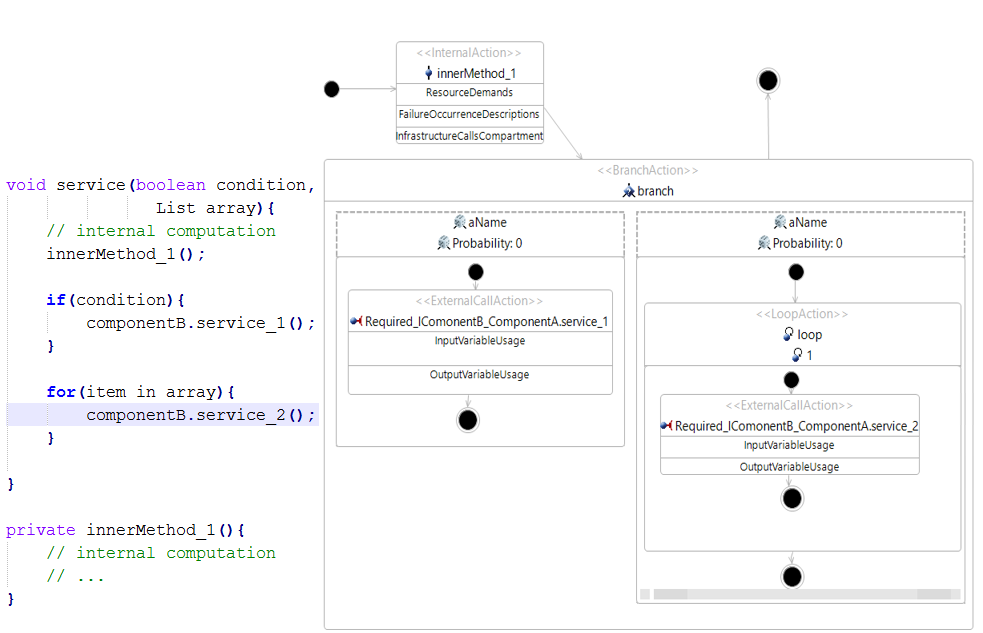
\includegraphics[width=0.9\textwidth]{figures/code_seff}
\caption{Example of source code and SEFF}
\label{fig:Example of source code and SEFF}
\end{figure}


\section{Vitruvius}
\label{sec:Vitruvius}

The Vitruvius approach is a view-based \cite{goldschmidt2012view} engineering approach, which was introduced in \cite{burger2013flexible, kramer2013view}.  Vitruvius can be used to keep the models of a system consistent. In Model Driven Engineering (MDE) \cite{thomas2005erzeugung}, the whole system can be represented by different models that describe different aspects of the system, even the source code of the system is seen as a model. These models can be changed separately and became inconsistent, for example if the source code of a system has changed, the architecture model of the system has to be also updated. In this case, architectures must capture the changes in the source code and update accordingly the associated architecture model. Therefore, Vitruvius performs this task automatically by defining consistency rules that define how the changes in a model must be transformed to another model.

Vitruvius uses views to make access to the models possible. This approach reduces the complexity of dealing with the whole models, because views present only a part of the model. Therefore, developers can focus only on the relevant parts of the system.

Vitruvius defines the so called Virtual Single Underlying Model (VSUM), which contains all information related to a system. VSUM contains the meta-models instances, that are used within a system. Moreover, Vitruvius provides the correspondence meta-model, which offers the possibility to map between correspondent elements of different model, like SEFFs in PCM and methods in Java source code.  

To enable the process of keeping models consistent within Vitruvius, developers should provide and implement two concepts defined by Vitruvius, namely Domains and Application. A Vitruvius Domain represents a defined meta-model in the system and provides information for its use within the Vitruvius framework. Vitruvius Domains can be reused, for example the Domain of Java meta-model can always be used in systems that are implemented using java. Vitruvius Applications determine the relation between two Domains. They specify how changes in a Domains meta-model instance should be transformed to the instance of another Domains meta-model instance. Vitruvius Applications can be also reused in many environments, if the are needed.

\subsection{Vitruvius VSUM}
\label{sec:Vitruvius VSUM}
In order to keep models instances consistent, Vitruvius approach uses the so-called Virtual Single Underlying Model (VSUM) which contains all information that represents the system Figure \ref{fig:vitruv_vsum}. The models in VSUM are accessible using views. Views are instances of view types and they can be used to manipulate model instances. Moreover, there are two kinds of view types, namely projectional view types or combining view types \cite{burger2013flexible}. Projectional view types allows to show information from one meta-model solely. Combining view types can be used to show information from diverse meta-models.

Models consistency in Vitruvius can be preserved using Consistency preservation rules. They describe how changes in one model should be transferred into changes in another model. Moreover, the Consistency Preservation Process uses these rules to create the models transformation that preserves the consistency.


\begin{figure}[h]
\centering
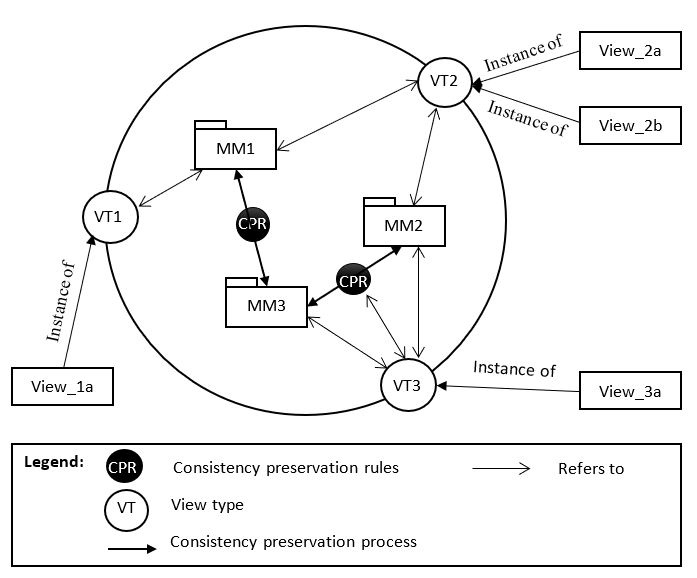
\includegraphics[width=0.9\textwidth]{figures/vitruv_vsum}
\caption{Overview of the Vitruvius VSUM and how model instances can be kept consistent}
\label{fig:vitruv_vsum}
\end{figure}

\subsection{Correspondence Meta-model}
\label{sec:Correspondence Meta-model}
The Correspondence Metamodel (CMM) is used within Vitruvius in order to describe the corresponding elements of two meta-models. Moreover, Vitruvius one instance of CMM can be used for each Vitruvius application. A Vitruvius application can have one or many meta-models instances.  In our approach, we use one CMM instance which has been created and used in the Coevolution approach. Furthermore, for the process of probes generation we will use the existing information in this instance that have been saved the Coevolution approach and add new information to it by extending the Coevolution approach.

Figure \ref{fig:correspondence_model} shows the Vitruvius Correspondence Meta-model. It's basically composed from two classes. The root class Correspondences contains the list of Correspondence. The class Correspondence is composed from two list of identifier references. The first list contains identifiers that reference models in one meta-model, while the second list contains identifiers that reference models in the other meta-model.

CMM is a generic and can be used for diverse meta-models. Therefore, in order to identify an element, the reference in the Correspondence has to be unique because only one concrete element needs to be identified for a given ID. For this purpose, the CMM uses the so-called Temporarily Unique Identifier (TUID) mechanism. TUID is a string that can identifies an element. It has to be calculated based on the properties of the element that it represents. The TUID is also used when an element needs to be retrieved from the correspondence model.    

\begin{figure}[h]
\centering
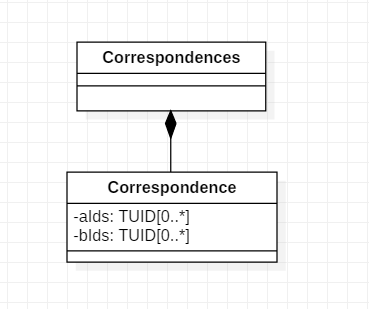
\includegraphics[width=0.6\textwidth]{figures/correspondence_model}
\caption{The Correspondence Meta-model of the Vitruvius Framework}
\label{fig:correspondence_model}
\end{figure} 

\section{Java Model Parser and printer}
\label{sec:Java Model Parser and printer}

Java Model Parser and Printer (JaMoPP) \cite{heidenreich2009closing} is a parser and printer for the Java language. JaMoPP defines a complete meta-model for the Java language based on the meta modeling language Ecore \cite{steinberg2008emf}. JaMoPP parser allows to parse a Java source code into a Java model, and the JaMoPP printer allows to print a Java model into Java source code. JaMoPP can convert Java source code into an EMF model, which can be manipulated using model driven techniques, like models transformation. Using JaMoPP, we can for example, parse a Java file, which contains Java source code, add new Java statements after or before an existing statement and print back the changes in the Java source code file. The creation of JaMoPP is based on EMFText \cite{heidenreich2009derivation}, which allows to define text syntax for languages described by an Ecore meta-model. 


\section{Automated Coevolution of Source Code and Software Architecture Models}
\label{sec:Automated Coevolution of Source Code and Software Architecture Models}
The approach of co-evolution of source code and component-based software architecture presented in \cite{langhammer2015co, langhammer2017automated} is based on the platform Vitruvius present above. It gives developers and architectures the possibility to keep the architecture and the source code of a software system consistent. The Consistency in this approach is kept in both directions, that means, if developers changed the source code of a system, the corresponding architecture will automatically be changed, and if architectures updated the architecture of the system, the source code will also automatically be updated. The co-evolution approach uses PCM models as architectures models.  Therefore, it describes the behavior of the source code in term of SEFF. Hence, a special objective of the co-evolution approach is to keep incrementally the behavior of the source code consistent with the source code itself. The incremental up-to-date of the behavior model of the source consists of only the part of the SEFF that corresponds to the changes performed in the source code. For example, if the developers update a service S of Component A, only the SEFF of the service S will be reconstructed but not the whole SEFF model of the system. 

The co-evolution approach uses two different concepts to preserve different modes consistent, namely model-driven engineering and change-driven engineering. Moreover, the co-evolution approach uses the concepts of Vitruvius to keep tracks of the models, that represents the system. 

The co-evolution approach considers all involved artifacts as models. Hence, the model-driven engineering is used in this approach as a main concept. In mode-driven engineering, all artifacts of the system are represented by models and the models are centric in the development process. That means, that the source code must be also represented within the co-evolution approach as a model. Therefore, in the case of Java, the co-evolution approach uses JaMoPP to parse the Java source code to a mode, on which the change-driven techniques can be applied, like model to model transformations.

The co-evolution approach uses change-driven engineering in order to reacts on changes, that the users perform on models, especially the architecture model and the source code model. These changes are monitored, converted in a Vitruvius change model and propagated. The propagated changes can be captured and transferred using consistency preservation rules to the target model. The consistency preservation rules are bidirectional and defined between the architecture meta-model and the source code meta-model.

The co-evolution approach was applied to the Palladio Component Model (PCM) as an architecture model and Java source code.  However, the concepts presented in this approach can be applied to other component-based architecture model, like UML component-diagrams, and other object-oriented languages. In the following, we will review the application of the co-evolution approach to PCM and Java source code and the steps, that are required to keep PCM models instances and Java source code consistent. 



Figure  \ref{fig:coevoloution approach} shows the steps, that are used to keep architecture models and the source code consistent:

\begin{itemize}
\item Step (0): users change either the PCM repository, the PCM system or the Java source code.  
\item Step (1): monitors capture changes on the models.
\item Step (2):  monitors trigger Vitruvius Framework and pass it the changes.
\item Step (3): based on these changes, the Vitruvius framework executes the consistency preservation transformations. 
\item Step (4): the transformations use information from the changes and the correspondence model to execute the preservation rules.
\item Step (5): the transformations update the models. 
\end{itemize}

When it comes to an automatic update of SEFF in step (5), the co-evolution approach executes an incremental SEFF reconstruction step instead of transformation. 


\begin{figure}[h]
\centering
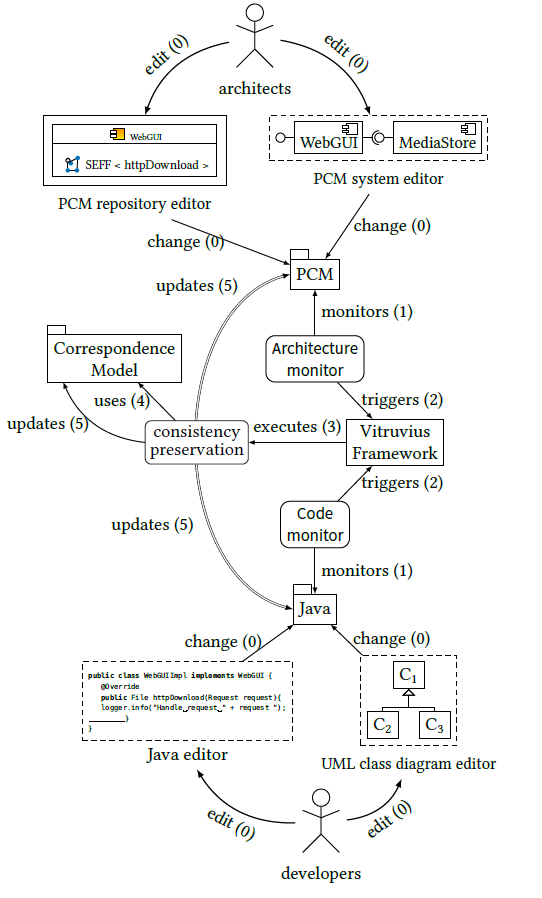
\includegraphics[width=0.9\textwidth]{figures/coevolution_approach}
\caption{The steps used in co-evolution approach to keep architecture models and the source code consistent \cite{langhammer2015co}}
\label{fig:coevoloution approach}
\end{figure}

\subsection{Incremental SEFF Reconstruction}
\label{sec:Incremental SEFF Reconstruction}
Langhammer has proposed in his Co-evolution approach an incremental SEFF reconstruction approach Figure \ref{fig:seff incremental reconst} which can build the SEFFs for only the changed parts of the source code. In contrast to SoMoX, the incremental SEFF reconstruction neither require the parsing of the complete project source code nor the SCDM. Moreover, the SEFF of the smallest unit that can be currently incrementally reconstructed is the SEFF of a method. 

The incremental SEFF reconstruction is integrated in the co-evolution approach that means it can use functionalities and information provides by Vitruvius. Moreover, the incremental SEFF reconstruction is done in change-driven way, that means change that happened in the source code are captured in a Vitruvius change model instance and can be treated in order to regenerate the SEFF of the method in which they belong. To classify the method calls which is necessary for SEFF reconstruction, Langhammer uses the current preservation rules and information from the Vitruvius correspondence model. More details on this step can be found in his thesis \cite{langhammer2017automated}.

\begin{figure}[h]
\centering
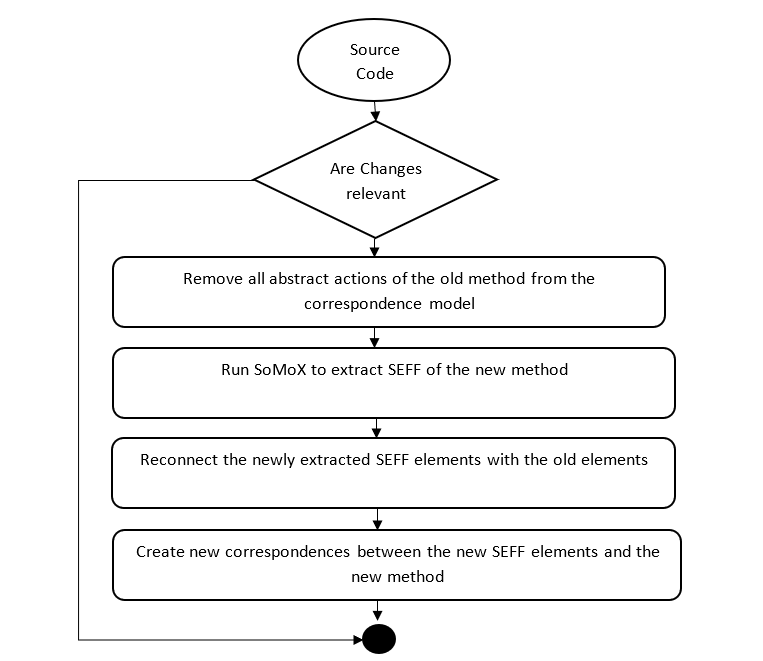
\includegraphics[width=0.9\textwidth]{figures/inscremental_seff_reconst}
\caption{Overview of the incremental reconstruction process of SEFF}
\label{fig:seff incremental reconst}
\end{figure}


\section{Kieker Monitoring Framework}
\label{sec:Kieker Monitoring}
Kieker is an extensible Java-based application performance monitoring and dynamic software analysis framework \cite{van2009continuous}. Figure \ref{fig:kieker} shows the architecture of Kieker framework. It's composed from two main components, namely the monitoring component and analysis component.   The analysis component can be used to read monitoring data, analyze and visualize them for a certain purpose, like generating UML sequence diagram, dependency graphs or Markov chains.

The monitoring component is responsible for source code instrumentation, data collection and data logging. The Monitoring probes are responsible for collecting the monitoring data and send them to the monitoring controller component, which instantiates a monitoring record for every probe. The Monitoring writer component receives the monitoring records from the monitoring controller and serialize them to the monitoring log/stream. 

A monitoring Record represents the measurement data gathered in a single measurement. Kieker provides the possibility to store different types of records for different types of probes. Kieker offers the possibility to create customized probes. We can create new probes either manually by extending the interface IKiekerMonitoringProbe or automatically by using the Instrumentation Record Language (IRL) \cite{jung2013instrumentation}. For example, in one record, we can store the signature and the response time of a method, in another record, we can persist the response time of specific number of statements inside a method.

A monitoring Probe represents the monitoring logic used to collect measurement data from the application. There are two ways to use probe within Kieker.  There is the manually instrumentation, which consists of mixing the instrumentation logic with the business logic of the application. Figure \ref{lst:kieker_manual_instr} show an example, in which the monitoring probe is implemented by mixing monitoring logic with business logic, in this example we create a probe that logs the name of the called service, the start time and end time. Kieker includes also probes based on Aspect Oriented Programming (AOP) \cite{kiczales1997j}, which helps to separates the instrumentation logic from the business logic. Kieker defines AOP based monitoring probes like OperationExecutionAspectAnnotation and OperationExecutionAspectAnnotationServlet. Figure \ref{lst:kieker_aop_instr} shows how the instrumentation looks like, when using AOP for probes implementation.

Using AOP to instrument the source code has the advantage of separating concerns. However, this technique has a limitation, when it comes to the monitoring of certain statements of inside a method, like monitoring the number of executions of a loop or the probability of a branch execution, because the annotation possibilities on these cases are out of box. 


\begin{figure}[h]
\centering
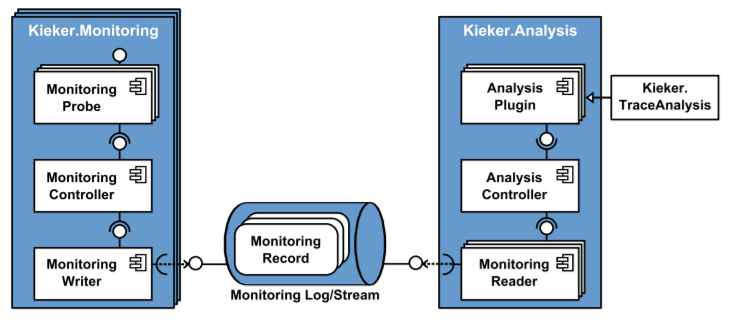
\includegraphics[width=0.9\textwidth]{figures/kieker}
\caption{Overview of the Kieker's architecture \cite{van2009continuous}}
\label{fig:kieker}
\end{figure}

\begin{lstlisting}[caption={Example of manual instrumentation of source code},label={lst:kieker_manual_instr}, captionpos=b, language=java] 
    final long tin = MONITORING_CONTROLLER.getTimeSource().getTime();
    // call of the service
    this.serviceA();
    final long tout = MONITORING_CONTROLLER.getTimeSource().getTime();
     // Create a new record and set values
    final MyResponseTimeRecord e = new MyResponseTimeRecord(
    "serviceA", tout, tin);
    // Pass the record to the monitoring controller
    MONITORING_CONTROLLER.newMonitoringRecord(e);
\end{lstlisting}


\begin{lstlisting}[caption={Example of a Kieker Probe using AOP},label={lst:kieker_aop_instr}, captionpos=b, language=java] 
    @OperationExecutionMonitoringProbe
    public void serviceA(){
       /*
        method content
       */
    }
\end{lstlisting}


\section{Source Code Model eXtractor}
\label{sec:Source Code Model eXtractor}
Source Code Model eXtractor (SoMoX) is a reverse engineering approach, which has been developed by Krogmann \cite{krogmann2012reconstruction}. SoMoX is able to reverse-engineer software component architectures. Moreover, SoMoX can extract a PCM repository from source code and creates a PCM system derived from the repository. The repository created by SoMoX contains mainly components, interfaces, roles and SEFFs. Thus, the results of reverse engineering of SoMoX depend strongly on the project implementation to reverse-engineer which means that SoMoX delivers best results, if the analyzed source code followed a component-based architecture.

In the following, we will review only the features of SoMoX that are involved in the context of this thesis. 

In order to create the architecture of a software system, SoMoX reverse-engineer the software system using the following steps:
\begin{itemize}
\item Parse the source code into a model.  
\item Detect components and interfaces using metrics.
\item Detect data types and signatures using metrics.
\item Reconstruct the SEFFs.
\end{itemize}

For the source code parsing in the first step, SoMoX uses JaMoPP to create an EMF model of the Java source code that can be manipulated. In this thesis, we will also use JaMoPP source code parsing and manipulation purpose.

For components and interfaces detection, SoMoX uses various source code metrics and combine them to determine detection strategies for architecture elements. These metrics must be given each a value between 0 and 100 by the user of SoMoX. The value of the metric tells SoMoX the impact factor, for example the value 0 of a metric means that the impact factor is low, whereas the value 100 of the metric means that the impact factor is high. 

The reconstruction of SEFFs which aims to reverse-engineer the statical behaviour of the source code is done by analysing the methods of the source code. This step has been extended by Langhammer \cite{langhammer2017automated} and its results are used in thesis. In the following, we will explain briefly how the reconstruction of SEFFs is done within SoMoX and how it was extended by Langhammer.
\subsection{Source Code Decorator Model}
\label{sec:Source Code Decorator Model}

The Source Code Decorator Model (SCDM) has been presented within the SoMoX approach (Section \ref{sec:Source Code Model eXtractor}).  SoMoX reverse-engineers the source code and can extracts the architecture models from it. Moreover, SoMoX can be used to extract the Palladio Component Model (PCM) from the Java Source Code. The SCDM is used to create trace links at the model level. The linking between the source code elements and the architecture model elements are needed in the reverse-engineering process. Therefore, the SCDM creates links between the source code elements and the PCM elements. Furthermore, due to the use of SCDM, the reverse-engineering process can be done without mixing the linking concerns with the domain specific language of the source code model and the architecture model.

The SCDM was also used in the Coevolution approach (Section \ref{sec:Automated Coevolution of Source Code and Software Architecture Models}) which keeps automatically the Java Source Code and the PCM models consistent during the system development. The SCDM was used to contain the information, which source code element is reverse-engineered into which architectural model element. For example, it contains the information, which classes are mapped into which component.

In our approach we will need the SCDM in order to map between the SEFF elements and the source code elements or the statements. As mentioned before, the instrumentation points in our approach are represented by the SEFF elements. Moreover, in order to insert the instrumentation code in the right location in the source code of the system, we need to know which SEFF elements corresponds to which source code statements. The SCDM offers this possibility by mapping between each SEFF element and the corresponding JaMoPP statements. 

In order to map between the SEFF elements and the JaMoPP statements, we do not need to implement this feature because it's done already in the Incremental SEFF Reconstruction Process (section \ref{sec:Incremental SEFF Reconstruction}) in the Coevolution approach. This process can monitor the changes within the source code and reconstructs incrementally the SEFF models. Moreover, the execution of this process requires the execution of the SoMoX in order to reverse-engineer the changed parts of the source code. The execution of SoMoX creates the SCDM which maps between the SEFF elements (like Branch Actions, Internal Actions, etc.) and the JaMoPP statements Figure \ref{fig:seff jamopp}.


\begin{figure}[h]
\centering
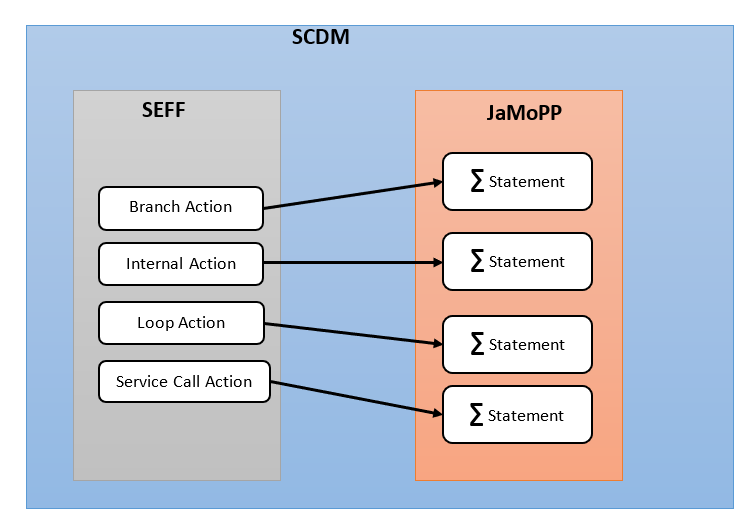
\includegraphics[width=0.9\textwidth]{figures/seff_jamopp}
\caption{Source Code Decorator Model (SCDM) maps between the SEFF elements and the corresponding JaMoPP statements}
\label{fig:seff jamopp}
\end{figure}

\subsection{SoMoX SEFFs Reconstruction}  
\label{sec:SoMoX SEFFs Reconstruction}
For SoMoX SEFFs reconstruction which is done in the last step of the reverse-engineering process, SoMoX uses two models which were created in the first and the second steps. The first model is the Java source code model which was created in the first step and the second is the so-called Source Code Decorator Model (SCDM) which was created in the second step. The SCDM contains the information that map between the source code model elements and the reverse-engineered architectural model elements.

In order to create the SEFF of a method, SoMoX analyses the source code of the method which was detected as a provided method of a component. This analysis is performed in two steps which are described in the following.

In the first step, the SoMoX visits all the method calls within the analysed method and classified them in three categories. The first category contains the component-external method calls which are considered as required roles. The second category contains library calls which considered as calls to a third-party library like java.lang. the second category contains the component-internal calls which are calls to the inner methods of the component. 

In the second step, SoMoX creates the SEFF for the method.  To do so, SoMoX visit again the statements in the source code of the method in order to find the following SEFF elements if they exist: ExternalCallActions, BranchActions, LoopActions and InternalActions. BranchActions and LoopActions are created for branches and loops. A Branch or a Loop is considered as BranchAction or LoopAction if it has an external method call, else it will be combined with an InternalAction.

\section{DevOps}
\label{sec:DevOps}
DevOps \cite{brunnert2015performance} is an agile development process which combines between development (Dev) and operations (Ops). The main goal of DevOps is to reduce the time between changes in the business process and the delivery of a solution to these changes. It achieves its goal by acting mainly on simplifying the communication between organizational and technical teams as well as introducing the automatization for the tasks that can be automated. 

\section{Continuous Integration of Performance Model}
\label{sec:Continuous Integration of Performance Model}
Continuous Integration of Performance Model (CIPM) is an approach proposed by Mazkatli and Koziolek \cite{mazkatli2018continuous} in order to extract incrementally and iteratively the Performance Model from the source code and enrich it by the Performance Model Parameters (PMPs). Furthermore, CIPM aims to keep the source code and the extracted Performance Model consistent during the system development. CIPM extends the Continuous Integration (CI) and the Continuous Deployment (CD) of the source code with a continuous integration of the performance model. 

To achieve that Mazkatli and Koziolek used the Coevolution approach developed by Langhammer (Section \ref{sec:Automated Coevolution of Source Code and Software Architecture Models}) which uses the Palladio Performance Model as a Performance Model and the Vitruvius Platform to keep incrementally and in a change-driven way the source code and the corresponding Performance Model consistent. CIPM uses likewise a change-driven way to enrich the extracted PM by the Coevolution process with PMPs. It defines the consistency rules that minimize the monitoring of the source code execution and the analysis overhead. In addition, it specifies a self-validation process that validates the estimated PMPs. To release that, CIPM automates four activities that are executed in each iteration \ref{fig:CIMP activities}. In this section we will describe only the first two activities because we based our work on them, more details on the other activities can be found in \cite{mazkatli2018continuous}.

The activities in CIPM are represented by the Reaction Language (RL) routines. RL is used in Vitruvius to describe the consistency rules and it's based on two concepts, namely reaction and routine. A reaction specifies changes and triggers a routine that contains the consistency rules that should be executed in reaction to these changes.  

The first activity in CIPM is responsible for updating the structure of the performance model, the usage model and the probes used in the activity two. The structure of the performance model is updated based on the work of Langhammer \cite{langhammer2015co}. The usage model is extracted incrementally from the test cases. For the probes generation CIPM specifies an Instrumentation Metamodel (IMM) and added it to VSUM. IMM contains and manages the instrumentation points and the weaving information based on Aspect-oriented Programming (AOP) \cite{kiczales1997j}. CIMP defines the consistency rules that keep the instrumentation model and the source code consistent. For example, a new probe can be added to the instrumentation model, when a part of the source code was added that corresponds to a new SEFF element. 

The second activity uses the probes from the first activity, instruments the source code and creates the monitoring data. For the monitoring data, CIPM specifies a Measurement Meta-model (MMM) and added it to VSUM. MMM describes the data structures of the different monitored data as well as the consistency rules to keep it consistent with the IMM. For example, after the monitoring phase is done, if a SEFF element had enough monitoring data, this element has to be deactivated in the instrumentation model. 

\begin{figure}[h]
\centering
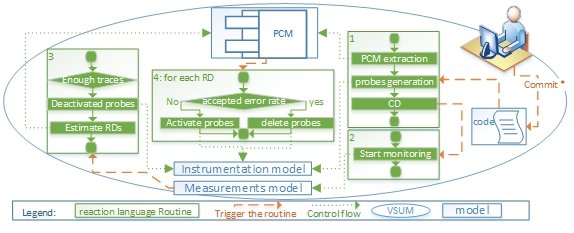
\includegraphics[width=0.9\textwidth]{figures/cipm}
\caption{CIMP activities \cite{mazkatli2018continuous}}
\label{fig:CIMP activities}
\end{figure} 

\subsection{Iterative Performance Model Parameter Estimation Considering Parametric Dependencies}
\label{sec:Iterative Performance Model Parameter Estimation Considering Parametric Dependencies}
Jägers has created his master thesis \cite{jagers2018Iterative} an approach that can estimate Performance Model Parameters taking into account the parametric dependencies. The approach is based on the vision presented by Mazkatli and Koziolek (Section \ref{sec:Continuous Integration of Performance Model}), it extends precisely the concepts introduced in the activities three and four in Figure \ref{fig:CIMP activities}. The approach is designed to make iteratively the estimation and thus reduce the overhead resulting from the estimation for the whole system. 

Jan uses the Palladio Performance model as a Performance Model for his approach. Since the Palladio Performance Model is expressed in terms of SEFF, Jan estimates the performance model parameters for loop iteration, resource demands, branch transitions and external call arguments. He specifies diverse predictive models for estimating Performance model parameters. He uses decision threes to create a predictive model for branch transitions. For loop iterations and resource demands he uses regression analysis. The predictive models are related with service call arguments. The predictive models can be transformed into stochastic expressions in order to use them for enriching performance model.

This approach uses as inputs the monitoring data that are generated from instrumenting and executing the source code that corresponds to the performance mode for which the estimation is done. The monitoring data are structured in records that contain diverse information about diverse source code elements like loop record, branch record response time record etc. Since the execution depends strongly on the monitoring data, in order to keep the estimation iterative, the monitoring must be also done iteratively. this includes also the fine-grained, automatic, iterative instrumentation of the source code. the instrumentation has to be fine-grained because the estimation requires specific information about the program elements like the number of loop execution, the response time of a specific source code that corresponds to an internal action. This thesis provides an approach that can generate iteratively the monitoring data for performance model. These monitoring data can be used by the approach of Jan to make the estimations.








%% LaTeX2e class for student theses
%% sections/conclusion.tex
%% 
%% Karlsruhe Institute of Technology
%% Institute for Program Structures and Data Organization
%% Chair for Software Design and Quality (SDQ)
%%
%% Dr.-Ing. Erik Burger
%% burger@kit.edu
%%
%% Version 1.3.2, 2017-08-01

\chapter{Thesis Statement}
\label{ch:Thesis Statement}
In this section, we will introduce our contribution to the subject of adaptive monitoring for performance model integration as well as the involved scientific challenges that must be solved in order to achieve the goals of our contribution. 

\section{Contribution}
\label{sec:Contribution}
The contribution of this thesis is an extension of the contribution presented in the approach CIPM (Section). Precisely, we focus in our contribution on the first and the second activity of the CIPM approach. \\

In order to contribute to the subject of adaptive monitoring for performance model integration, we’ve created an approach that takes into account two properties. The first property is the adaptive monitoring which means that the probes which are responsible for logging the monitoring data are capable to be activated and deactivated during the monitoring phase. The meaning is that once we have collected enough monitoring data of a probe, the probe must be deactivated because more monitoring data is not necessary and can influence the performance of the monitoring.   Furthermore, we adapted our approach to the fine-grained monitoring. This is required, when the used performance model needs performance model parameters (like Resource Demands RDs, loop execution number, the probability of selecting a branch). Therefore, we adapted our approach to monitor the response time of computation, the number of execution of loops, the executions of branches and the parameters of a method calls.\\

The second property is the monitoring for continuous integration of performance model. The continuous integration of performance model in this context means the incremental update of the performance model in each iteration. The incremental update of the performance model includes the possibility to keep first of all the status of the performance model in the previous iteration and then update it with the information provided within the current iteration. The opposite of that will be to extract the whole performance model in each iteration which will lead to two issues. The first issue is that the extracted performance model in an iteration will not be saved in the next iteration which will cause the second issue. Since the iterations do not consider the modification done in the previous ones, the whole system will have to monitored in every iteration in order to provide the required monitoring data for the new extracted performance model. Hence, in the case of huge Enterprise Applications EAs monitoring the whole system in every iteration will cause a monitoring overhead which is unfeasible and that is the second issue. \\

To guarantee the monitoring for performance model integration, we’ve made the following decisions: 
\begin{itemize}
\item We used the Palladio Performance Model as a performance model.  
\item We used Vitruvius to support the model-driven development in our approach.
\item We used the Coevolution approach for the continuous creation of performance model. 
\item We created an instrumentation model to persist the generated probes.
\end{itemize}

\section{Scientific challenges}
\label{sec:Scientific challenges}
in this section, we will identify the scientific challenges that we will resolve in order to achieve the goals of this thesis. 
\begin{itemize}
\item \textit{what are the steps necessary to generate the probes and instrument automatically the source code for monitoring?} \\
In order to monitor the source code of a system, the system must be firstly instrumented using the needed probes. The instrumentation in our approach is done automatically based of the generated probes during the system development. Moreover, the processes of probes generation and the source code instrumentation can be executed independently. Therefore, we need to define the necessary steps to execute these processes and how they change information between them.

\item \textit{what are the probes that must be generated for the monitoring?}\\
The definition of probes for monitoring is based on the monitoring data needed by the performance model. Since we used Palladio Performance Model, we have to define probes that provide monitoring data that can be used by the Palladio Performance Model.
 
\item \textit{What are the models required to support the iterative and adaptive monitoring?}\\
In order to enable the iterative and the adaptive monitoring for continuous performance model integration. As mentioned before, we extend the coevolution approach which uses models like PCM, Java and Correspondence Model. Therefore, we need to use the information provided by the existing models and define new models for persisting the information that are not provided by the existing model.

\item \textit{What are the alternatives of the source code instrumentation for monitoring?}\\
The best way to instrument the source code of a system is to use Aspect oriented Programming (AOP) because it separates the instrumentation logic from the business logic which simplify the application maintenance. However, AOP is based on annotations which can not be used for all kind of probes. For example, we can not use AOP annotation to monitor the number of executions of a loop. Therefore, we need to find alternatives that enable the source code instrumentation without changing the original source code of the system. Otherwise, mixing the original source code with instrumentation code will make the readability of the source code infeasible for the user. 

\item \textit{What level of incremented update of performance model can we reach?} \\
Here, we define two levels of incrementation. In the first level, the performance model will be updated based on the changed services. In the second level, it will be updated based on the changed parts of the service. The difference between the first and the second level is that in the first level if a service has changed the SEFF of the service will newly recreated. Therefore, the old elements of this SEFF will be lost with their parameters. In the second level, the unchanged old elements in SEFF will be kept, the new elements will be added and the deleted elements will be deleted. The Coevolution approach has reached the first level. Thus, we will extend to reach the second level of incrementation.


\end{itemize}

%% LaTeX2e class for student theses
%% sections/content.tex
%% 
%% Karlsruhe Institute of Technology
%% Institute for Program Structures and Data Organization
%% Chair for Software Design and Quality (SDQ)
%%
%% Dr.-Ing. Erik Burger
%% burger@kit.edu
%%
%% Version 1.3.2, 2017-08-01


\chapter{An Approach for Adaptive Monitoring for Continuous Performance Model Integration}
\label{ch:An Approach for Adaptive Monitoring for Continuous Performance Model Integration}
In this chapter, we will introduce our approach for adaptive monitoring for continuous performance model integration. 

\section{Context of our approach}
\label{sec: Context of our approach}
As mentioned before, our approach is part of the CIPM vision (section 8) which extends the agile and DevOps process and provides them with iterative and incremental Performance Model. Moreover, the Performance Models in CIPM are enriched with Performance Model Parameters. In the following, we will briefly depict and describe the process and the context in which our approach takes place.\\

Figure \ref{fig:Context of our approach} shows the process in which our approach takes place. this process is based on Vitruvius (section 2) which means its elements are either models or transformations. The Java code in \ref{fig:Context of our approach} is represented by a JaMoPP model. When the developer commits changes on this model, two transformations will be triggered. The first one is the Coevolution process of Langhammer (section 5) which keeps the Source Code and the models in the Palladio Component Model consistent, mainly the repository and the SEFF Model. The second Transformation is our Transformation which is specified for keeping the Source Code and the Instrumentation Model consistent. We proposed the Instrumentation Model in order to persist the Probes that will be required for instrumenting the Source Code.\\

When the system under development is deployed, our Instrumentation Process will be triggered. This process receives as inputs the Probes from the Instrumentation Model and the Source Code of the System. It delivers afterwards the instrumented Source Code as a JaMoPP Model. After the instrumentation process has been finished, the instrumented Source code will be executed and monitored.  The information provided by monitoring are encapsulated in a Measurement Model which describes the needed monitoring records.  After the monitoring has been finished the Parameters Estimation Process (section 9) will be triggered. it uses the information in the Measurement Model to estimate the Performance Model Parameters and updates accordingly the SEFF Model in the Palladio Component Model. Afterwards, the user can use the updated Performance Model to simulate and evaluate the performance of the system. \\


\begin{figure}[h]
\centering
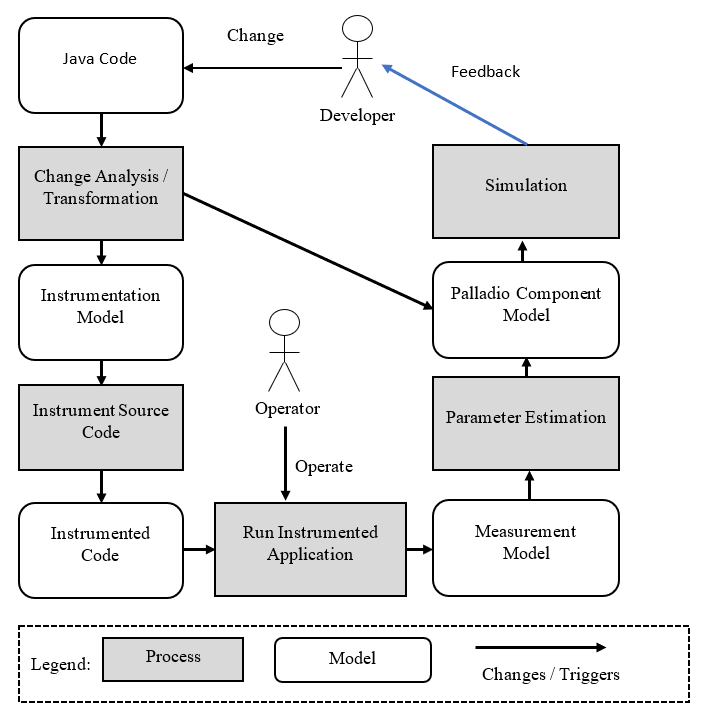
\includegraphics[width=0.9\textwidth]{figures/approach_context}
\caption{Context of our approach}
\label{fig:Context of our approach}
\end{figure}


\section{Monitoring Probes}
\label{sec:Monitoring Probes}
Monitoring Probes are responsible for collecting monitoring information from the system. Furthermore, they can be specified based on the needed monitoring information. For example, if we need to monitor the response time of a service and the number of execution of loops, we can specify two monitoring probes, one probe for the response time and the other for loops execution number. \\

In our approach, we want to provide monitoring information for Palladio Performance Model which are described in terms of SEFF (section 1.2).   SEFF Model is composed from four main elements which inherit from the so-called Abstract Action, namely Internal Action, Branch Action, Loop Action and Service Call Action. In other words, we should specify probes that provide these elements with the needed monitoring information. Therefore, we defined a monitoring probe for each SEFF element Figure 2. The monitoring information that we need to produce for SEFF elements are described in (section 1.3) under monitoring records.  \\

For the monitoring purpose, we used the Kieker Monitoring Framework (section 6) which offers the possibility to define new monitoring probes based on the needed monitoring records.\\

\begin{figure}[h]
\centering
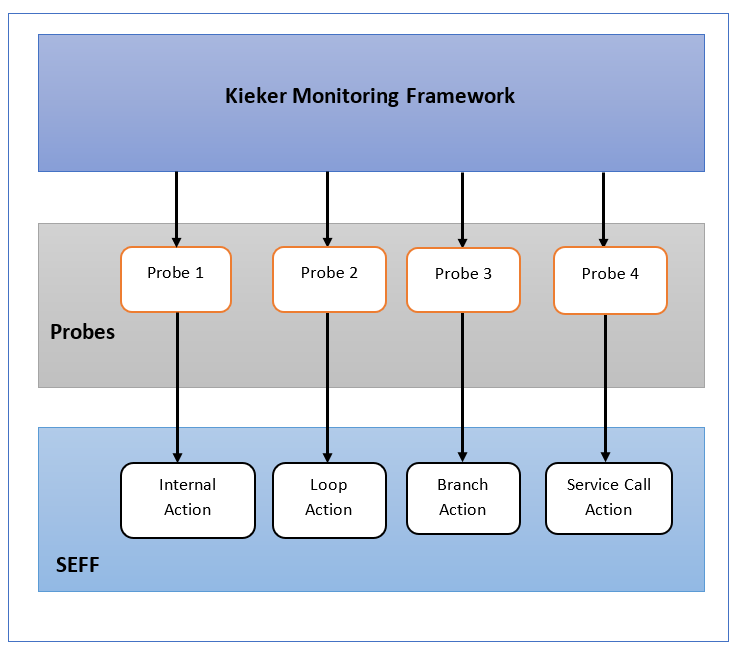
\includegraphics[width=0.9\textwidth]{figures/probes}
\caption{Specified Monitoring Probes in our Approach}
\label{fig:Specified Monitoring Probes in our Approach}
\end{figure}

\section{Monitoring Records}
\label{sec:Monitoring Records}
In order to create monitoring probes (section 1.2), one must define first of all   the needed monitoring information. in our case, we defined monitoring probes for SEFF model which are based on the monitoring records in Figure 3. \\

Figure 3 shows an UML Class Diagram that describe the monitoring records. It provides extra information that are needed for the purpose of performance model parameters estimations. The abstract class RecordWithSession specifies a sessionID attribute that helps to identify the monitoring information based on sessions.  The abstract class ServiceContextRecord adds a serviceExecutionID attribute that helps to reference a ServiceCallRecord.\\

All records are identified via their ids. The id of each record can be provided by the used monitoring framework. However, in order to be able to use these records for SEFF models we’ve used for each record the id of the corresponding SEFF element. \\

For internal actions which express internal computation, we want to know the time consumed by them. Therefore, we need to log the id of the internal action, start time and stop time. \\

For Loops, we need to recognize the number of executions of a loop. The same thing for branches, we log the id of the executed branch in order to realise if the branch was executed or not. \\

As to service calls, we need to locate them in which service are called, we need also to provide the response time and the parameters they are given. The parameters of services are given in a JSON format.\\

\begin{figure}[h]
\centering
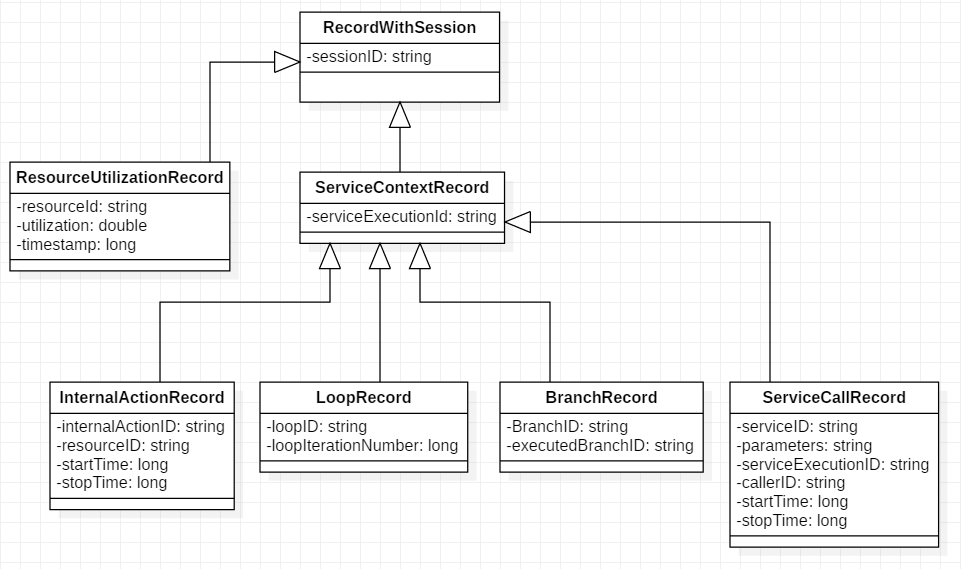
\includegraphics[width=0.9\textwidth]{figures/records}
\caption{UML class diagram that shows the monitoring information required by SEFF models}
\label{fig:records}
\end{figure}

\section{Adaptive Instrumentation}
\label{sec:Adaptive Instrumentation}
In this section, we will introduce the meaning of Adaptive Monitoring in our approach as well as the main concepts used in order to achieve that.\\

As mentioned before, our approach is addressed to iterative development processes like DevOps. In this context, Adaptive Instrumentation means that only the parts of the source code that have been changed in the current iteration will be monitored. \\

Based on this definition, we should be able to generate instrumentation points during the development phase. In order to do this, we decided to use two main concepts which are model-driven engineering and change-driven engineering. Moreover, our approach is based on the Coevolution approach which itself uses these two concepts to keep the source code and the architecture models consistent. Precisely, the Coevolution approach uses change-driven consistency preservation in order to keep the Java source code and SEFF models consistent. Changes in the source code model are monitored and transformed to changes in the SEFF model based on defined consistency-preservation rules. \\

In order to achieve an adaptive instrumentation in our approach, we’ve defined and Instrumentation Model which contains the instrumentation points. Moreover, we defined a transformation that monitored changes in the source code model and creates the corresponding instrumentation points in the instrumentation model. \\

In order to keep the source code and the instrumentation model consistent, we've used Vitruvius Framework which makes it possible to keep models instances consistent based on models changes. 

\section{Adaptive Monitoring}
\label{sec:Adaptive Monitoring}
Adaptive Monitoring means that the monitoring probes can be activated and deactivated based on the existing monitoring information. this is needed when we’ve collected enough monitoring information for some probes but they still can log monitoring information which is not needed and which can lead to monitoring and performance model parameters estimations overhead.  Therefore, adaptive monitoring can help to reduce the monitoring overhead by reducing the number of monitoring probes. \\

In order to achieve Adaptive Monitoring in our approach, we’ve added an attribute for the monitoring probes that defines their activeness. That means, monitoring probes are checked during the monitoring phase and they can log monitoring information only if the are activated. The deactivation of the probes can be done for example, when we've realised that the current monitoring information for these probes are enough for the performance model parameters estimation.\\

\section{Instrumentation Model}
\label{sec:Instrumentation Model}
The Instrumentation Model was originally presented in the approach of Manar and Koziolek \cite{mazkatli2018continuous} on which we based our approach. 

The Instrumentation Model (IM) Figure \ref{fig:im} is one of the Contribution of this thesis in Vitruvius. IM is responsible for describing and managing the instrumentation points. Moreover, we've defined IM in order to achieve the Adaptive Instrumentation (Section \ref{sec:Adaptive Instrumentation}) and Adaptive Monitoring (Section \ref{sec:Adaptive Monitoring}).\\

IM is composed from two elements, AppProbes which represents the model root and the element Probe which represents an instrumentation point. The element Probe corresponds to a SEFF abstract action which can be an Internal Action, a Branch Action, a Loop Action or a Service Call Action.\\

As mentioned before, we’ve used Vitruvius in order to keep the source code and the IM consistent. We've also extended the Coevolution approach which uses also Vitruvius to keep the Java source code and the architecture models consistent. The Coevolution approach uses an instance of the SEFF model in which our probes are stored. Therefore, in order to avoid redundant information within Vitruvius, we've decided to store only the Ids of these probes which give us the possibility to return them when they are needed. Moreover, since the probes represent concretely the four above mentioned abstract actions of SEFF, the id of a probes is named abstractActionID. Furthermore, we've added a boolean attribute to the monitoring probes in order to enable to adaptive monitoring. \\

\begin{figure}[h]
\centering
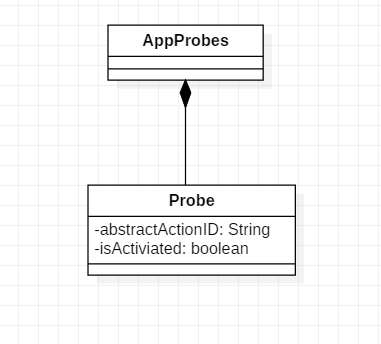
\includegraphics[width=0.5\textwidth]{figures/im}
\caption{UML Class Diagram that represents the Instrumentation Model}
\label{fig:im}
\end{figure}


\section{Approach}
\label{sec:approach}
In this section we will briefly introduce our approach as well as the context in which our activities will be executed. Further details on these activities will be presented in the next chapters.\\

our approach is developed in the context of the iterative development process DevOps. Therefore, Figure \ref{fig:devops_approach} gives an overview of the activities of our approach and in which DevOps phase they can be executed. The green color indicates processes or model in which our algorithms are executed. \\

In our approach we've defined to main processes. The first one is responsible for collecting the instrumentation points or the probes. It must be executed during the development phase. It uses information from Vitruvius and it's based on the Coevolution approach. The Coevolution approach keeps the source code and the SEFF model consistent and provides us with information that help to gather the probes. Vitruvius is used to keep the source code model and the Instrumentation Model consistent. The generated probes are saved and managed in the Instrumentation Model. For more details on the probes generation process, look at the chapter (Probes Generation Process).\\

The second process is the instrumentation process which can be executed at any time. Once it's executed, it takes the probes from the Instrumentation Model and insert the instrumentation source code in the source code of the system based on the types of the probes (Figure 2). However, if the monitoring will be firstly done in the monitoring phase of DevOps, this process can be automatically triggered at the Continuous Deployment phase. For more details on our instrumentation process look at the chapter (Source Code Instrumentation Process).\\

In the monitoring phase, the instrumented system can be executed in order to log monitoring information. Moreover, in order to achieve an adaptive monitoring, the monitoring probes execute a self-checking for their activeness. Therefore, the monitoring code uses information from the Instrumentation Model in order to check if probes are activated of deactivated and thus if they can log or not. \\


\begin{figure}[h]
\centering
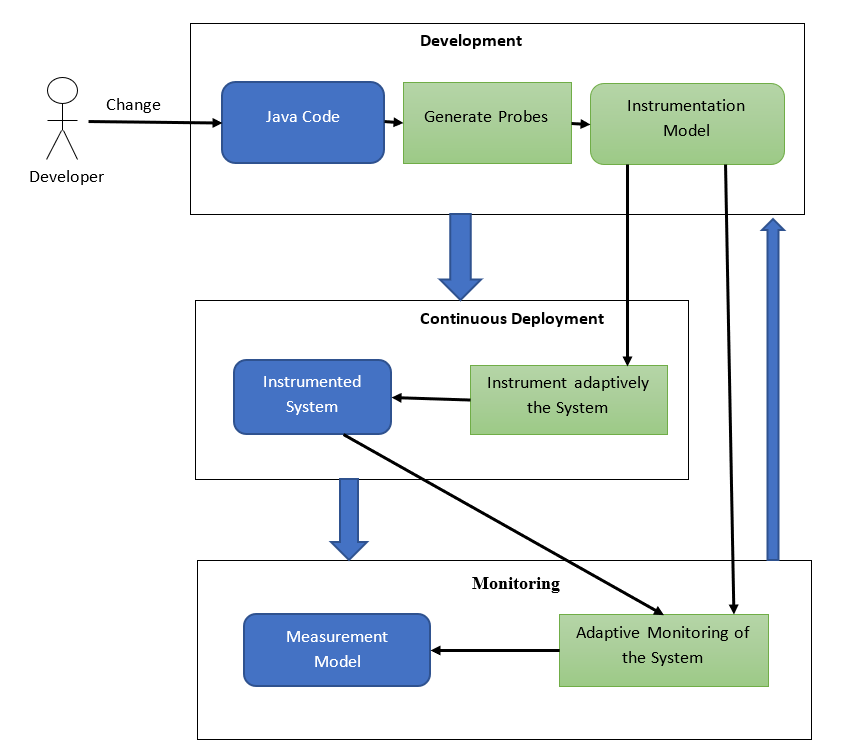
\includegraphics[width=0.9\textwidth]{figures/devops_approach}
\caption{Overview of our Approach Activities in DevOps context}
\label{fig:devops_approach}
\end{figure}

\section{Monitoring Probes Generation Process}
\label{sec:Monitoring Probes Generation Process}
As mentioned before, we used the Vitruvius Framework and change-driven approach to create the probes in order to achieve the adaptive instrumentation. Moreover, we showed that the generation of the monitoring probes is equivalent to keeping the source code model and the instrumentation model consistent. the consistency between these models is realised within Vitruvius.\\

In this section, we will introduce our approach for the monitoring probes generation as well as the collection of the information that is needed for the instrumentation process. In section \ref{sec:Terminology}, we introduce the concepts that are used in our approach. In section \ref{sec:The Vitruvius VSUM of our approach}, we present the Vitruvius VSUM of our approach. In section \ref{sec:Collecting Information for the Transformation}, we describe how we collect the information that we need in our approach and the transformation that keeps the source code and the instrumentation model consistent. In section \ref{sec:Limitation}, we provided an overview of the limitation of our approach.\\

\section{Terminology}
\label{sec:Terminology}
In this section, we present the terminologies and the concepts we use to achieve the goals of our approach. 

\subsection{Source Code Decorator Model}
\label{sec:Source Code Decorator Model}

The Source Code Decorator Model (SCDM) has been presented within the SoMoX approach (section 7 in foundation).  SoMoX reverse-engineers the source code and can extracts the architecture models from it. Moreover, SoMoX can be used to extract the Palladio Component Model (PCM) from the Java Source Code. The SCDM is used to create trace links at the model level. The linking between the source code elements and the architecture model elements are needed in the reverse-engineering process. Therefore, the SCDM creates links between the source code elements and the PCM elements. Furthermore, due to the use of SCDM, the reverse-engineering process can be done without mixing the linking concerns with the domain specific language of the source code model and the architecture model.\\

The SCDM was also used in the Coevolution approach (section 5 in foundation) which keeps automatically the Java Source Code and the PCM models consistent during the system development. The SCDM was used to contain the information, which source code element is reverse-engineered into which architectural model element. For example, it contains the information, which classes are mapped into which component.\\

In our approach we will need the SCDM in order to map between the SEFF elements and the source code elements or the statements. As mentioned before, the instrumentation points in our approach are represented by the SEFF elements. Moreover, in order to insert the instrumentation code in the right location in the source code of the system, we need to know which SEFF elements corresponds to which source code statements. The SCDM offers this possibility by mapping between each SEFF element and the corresponding JaMoPP statements. \\

In order to map between the SEFF elements and the JaMoPP statements, we do not need to implement this feature because it's done already in the Incremental SEFF Reconstruction Process (section 7.2 in foundation) in the Coevolution approach. This process can monitor the changes within the source code and reconstructs incrementally the SEFF models. Moreover, the execution of this process requires the execution of the SoMoX in order to reverse-engineer the changed parts of the source code. The execution of SoMoX creates the SCDM which maps between the SEFF elements (like Branch Actions, Internal Actions, etc.) and the JaMoPP statements Figure \ref{fig:seff jamopp}.


\begin{figure}[h]
\centering
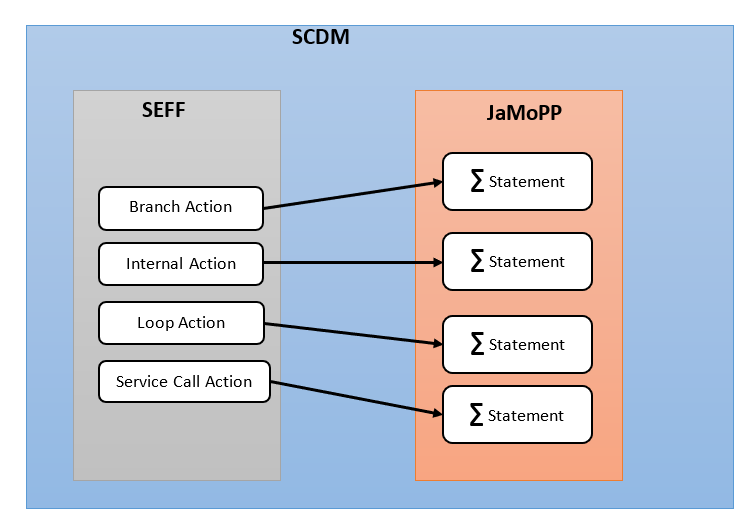
\includegraphics[width=0.9\textwidth]{figures/seff_jamopp}
\caption{Source Code Decorator Model (SCDM) maps between the SEFF Elements and the corresponding JaMoPP statements}
\label{fig:seff jamopp}
\end{figure}



\subsection{Correspondence Meta-model}
\label{sec:Correspondence Meta-model}
The Correspondence Metamodel (CMM) is used within Vitruvius in order to describe the corresponding elements of two meta-models. Moreover, Vitruvius one instance of CMM can be used for each Vitruvius application. A Vitruvius application can have one or many meta-models instances.  In our approach, we use one CMM instance which has been created and used in the Coevolution approach. Furthermore, for the process of probes generation we will use the existing information in this instance that have been saved the Coevolution approach and add new information to it by extending the Coevolution approach.\\

Figure \ref{fig:correspondence_model} shows the Vitruvius Correspondence Meta-model. It's basically composed from two classes. The root class Correspondences contains the list of Correspondence. The class Correspondence is composed from two list of identifier references. The first list contains identifiers that reference models in one meta-model, while the second list contains identifiers that reference models in the other meta-model.\\

CMM is a generic and can be used for diverse meta-models. Therefore, in order to identify an element, the reference in the Correspondence has to be unique because only one concrete element needs to be identified for a given ID. For this purpose, the CMM uses the so-called Temporarily Unique Identifier (TUID) mechanism. TUID is a string that can identifies an element. It has to be calculated based on the properties of the element that it represents. The TUID is also used when an element needs to be retrieved from the correspondence model.    

\begin{figure}[h]
\centering
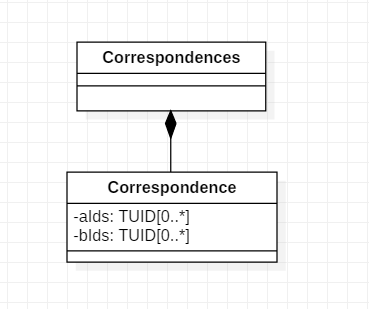
\includegraphics[width=0.9\textwidth]{figures/correspondence_model}
\caption{The Correspondence Meta-model of the Vitruvius Framework}
\label{fig:correspondence_model}
\end{figure}



\subsection{Vitruvius VSUM}
\label{sec:Vitruvius VSUM}
In order to keep models instances consistent, Vitruvius approach uses the so-called Virtual Single Underlying Model (VSUM) which contains all information that represents the system Figure \ref{fig:vitruv_vsum}. The models in VSUM are accessible using views. Views are instances of view types and they can be used to manipulate model instances. Moreover, there are two kinds of view types, namely projectional view types or combining view types \cite{burger2013flexible}. Projectional view types allows to show information from one meta-model solely. Combining view types can be used to show information from diverse meta-models.\\

Models consistency in Vitruvius can be preserved using Consistency preservation rules. They describe how changes in one model should be transferred into changes in another model. Moreover, the Consistency Preservation Process uses these rules to create the models transformation that preserves the consistency.\\


\begin{figure}[h]
\centering
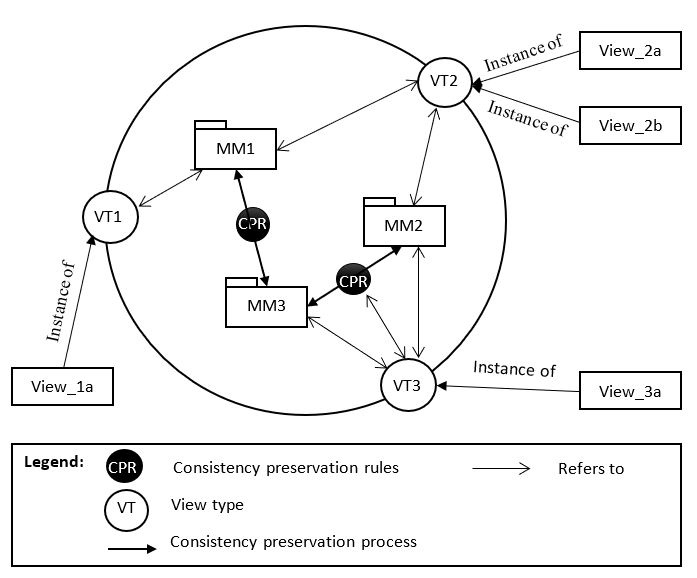
\includegraphics[width=0.9\textwidth]{figures/vitruv_vsum}
\caption{Overview of the Vitruvius VSUM and how model instances can be kept consistent}
\label{fig:vitruv_vsum}
\end{figure}



\section{The Vitruvius VSUM of our approach}
\label{sec:The Vitruvius VSUM of our approach}

In this section, we will present the VSUM of our approach in order to generate the monitoring probes. We will precisely extend the VSUM Figure (VSUM in foundation) defined by the Coevolution approach.\\

As mentioned above, our approach extends the Coevolution approach, which keeps the source code and the architecture consistent. The VSUM in the Coevolution approach is composed from the following models:
\begin{itemize}
\item Palladio Component Model: it represents the architecture models.
\item JaMoPP Model: it represents the source code of the system.
\item Correspondence Model: it links between diverse model elements.
\end{itemize}
Moreover, the steps that are used to keep these models consistent are described in (section 5 in foundation). \\

In order to use Vitruvius for the adaptive monitoring purpose, we added an Instrumentation Meta-model (Section \ref{sec:Instrumentation Model}) that saves the monitoring probes and keeps them consistent with the source code. Figure \ref{fig:extended_vsum} shows our VSUM which is extended from the VSUM of the Coevolution approach. The steps described in (section 5 in foundation) are kept the same. However, we added a transformation (Section \ref{sec:Keeping the Source Code and the Instrumentation Consistent}) in the step (5) which keeps the Java source code and the instrumentation model consistent. 

\begin{figure}[h]
\centering
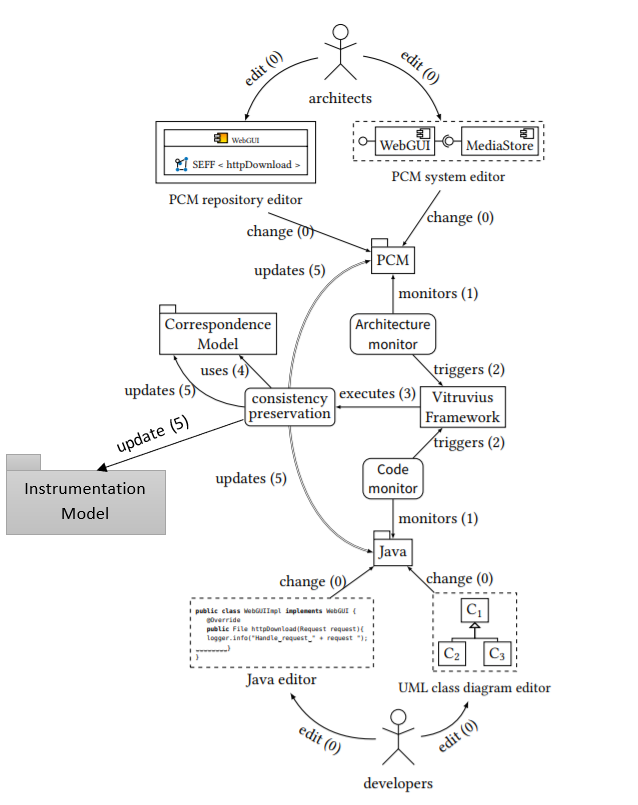
\includegraphics[width=0.9\textwidth]{figures/extended_vsum}
\caption{Overview of the Vitruvius VSUM of our approach, we extended the VSUM of the Coevolution approach}
\label{fig:extended_vsum}
\end{figure}

\section{Monitoring probes generation}
\label{sec:Monitoring probes generation}
In this section, we will introduce the process that we used to create the monitoring probes based on the Vitruvius Framework. This process is divided into two steps. The first step consists of collection the information that is useful for our transformation that keeps the source code and the Instrumentation Model consistent. the second step is the execution of this transformation.

\subsection{Collecting Information for the Transformation}
\label{sec:Collecting Information for the Transformation}
In this section, we present the process used to collect information. this information is can be used in the Instrumentation Process and for executing the transformation that generates the monitoring probes and keeps the source code and the instrumentation model consistent.\\

In order to execute our transformation, we need to know the new or the updated probes (SEFF elements).  For the Instrumentation Process we need the correspondence between the SEFF elements and corresponding JaMoPP statements. This information should be provided in each change of the source code. \\

In order to get this information, we used the information provided by the Incremental Reconstruction Process of SEFF (section 7.2 in foundation). This process reconstructs incrementally the SEFF of a service if its source code has been changed. Moreover, the SEFF elements are linked with the corresponding services in the Correspondence Model and can be retrieved from our transformation.\\

The second information that we need is the correspondence between the SEFF elements and source code. this information can be also provided by the SEFF reconstruction process. As described in (section 7.2 in foundation), the SoMoX is executed to reverse-engineer the changes service and creates its SEFF. SoMoX creates also the Source Code Decorator Model (SCDM) (Section \ref{sec:Source Code Decorator Model}) which contains links the SEFF elements of the service and the corresponding JaMoPP statements. Moreover, in order to make this information useful in our instrumentation process, we should make it accessible from outside of the SEFF reconstruction application. Therefore, we extended the SEFF reconstruction process with a new step that transforms the linking between the SEFF elements and the JaMoPP statements from SCDM into correspondences in the correspondence model Figure \ref{fig:seff_reconst_extension}. \\


\begin{figure}[h]
\centering
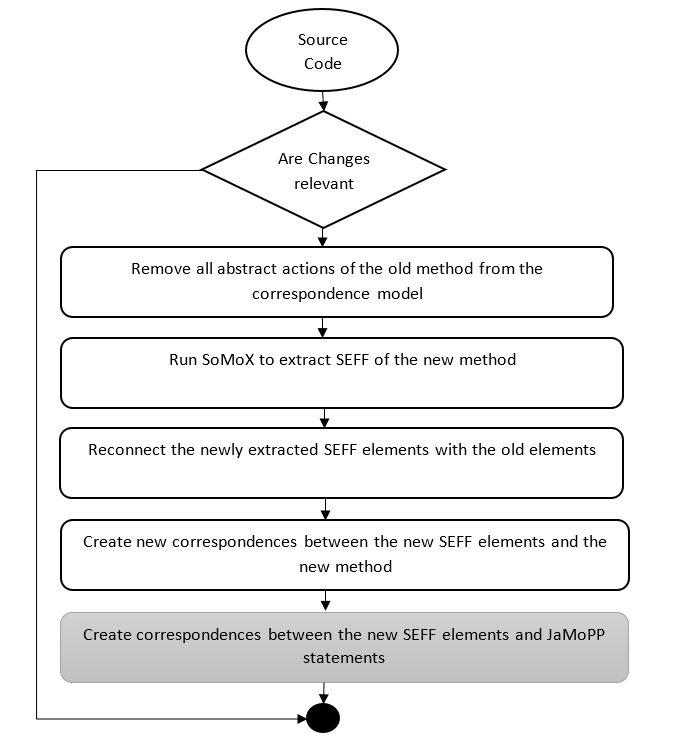
\includegraphics[width=0.9\textwidth]{figures/seff_reconst_extension}
\caption{The extended Incremental Reconstruction Process of SEFF}
\label{fig:seff_reconst_extension}
\end{figure}


\subsection{Keeping the Source Code and the Instrumentation Consistent}
\label{sec:Keeping the Source Code and the Instrumentation Consistent}
In this section, we present our transformation that keeps the source code and the Instrumentation Model (Section \ref{sec:Instrumentation Model}) consistent.\\

In order to generate the monitoring probes in our approach, we should preserve the consistency of the source code and the instrumentation model. Therefore, we created a transformation that transfers changes in the source code into changes in the instrumentation model. This transformation is executed when the source code has been changed.\\

In order to execute our transformation, we need to know the old service and its SEFF elements as well as the new service and its SEFF elements. This information can be obtained from the Correspondence Model after the Coevolution has been executed. Therefore, the Coevolution approach and our transformation are executed asynchronously. That means, we execute firstly the Coevolution approach in order to collect the information for our transformation then we execute our transformation based on this information.\\

The consistency preservation rules in our transformation are simple. When the source code has been changed and the changes are relevant, we delete the old probes of the old service from the instrumentation model and we add the new probes of the new service in the instrumentation model. Moreover, the new added probes are by default activated (Section \ref{sec:Monitoring Probes}). \\

\section{Adaptive Instrumentation Process}
\label{sec:Adaptive Instrumentation Process}
bla bla bal
\subsection{Design}
\label{sec:Design}
bla bla bal
\subsection{Inputs}
\label{sec:Inputs}

Figure \ref{fig:approach_design} shows an overview of the inputs and the output of our Instrumentation Process. It receives three Inputs. First of all, the source code of the system which we want to monitor. secondly, The Correspondence Model which contains correspondences between the services and their SEFFs as well as correspondences between the SEFF elements and the corresponding JaMoPP statements. Finally, the Instrumentation Model which contains the instrumentation points that we should use to instrument the source code. 

\begin{figure}[h]
\centering
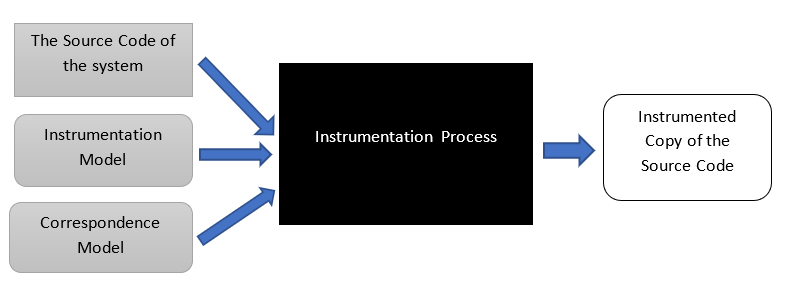
\includegraphics[width=0.9\textwidth]{figures/approach_design}
\caption{The inputs and the output of the instrumentation process, the output is an instrumented copy of the original source code of the system}
\label{fig:approach_design}
\end{figure}

\subsection{Output}
\label{sec:output}

The output of the Instrumentation process is an instrumented version of the source code of the system.  This instrumentation is based on the monitoring probes defined in (section Probes in the chapter approach). Moreover, there are two ways to instrument the source code. The first alternative consists of using the Aspect Oriented Programming which separate the instrumentation code from the source code of the system. The second alternative consists of mixing the instrumentation code with the source code of the system. Furthermore, we showed in (Section Kieker in  foundation) that the first alternative can not be used in our approach because of the fine-grained monitoring probes that we defined in our approach (section monitoring probes in the chapter approach). Therefore, we decided to use the second alternative in our instrumentation approach.\\

\textbf{Alternative of the instrumentation process outputs}\\
As mentioned above, in order to do the source code instrumentation, we decided to mix between the source code and the instrumentation logic.  Here, we distinguish also between two alternatives for instrumenting the source code of the system. The first alternative consists of instrumenting the original source code of the system. The second alternative consists of making a copy of the original source code of the system and instrument it. We decided to use the second alternative in our instrumentation process. \\

\textbf{Instrumentation of a copy of the source code}\\
The reason why we decided to use the second alternative to instrument the source code was due to the readability of the original source code. Moreover, if we instrumented the original source code of the system, we will reduce its readability and make the maintenance more difficult in the feature for programmers. Figure 2 shows an instrumented version of the source code in Figure( code in foundation). As we can see, the readability of the source code has become difficult and the maintenance will be also hard to do. Therefore, we decided the instrument a copy the original system in order to receive the monitoring information.


\begin{figure}[h]
\centering
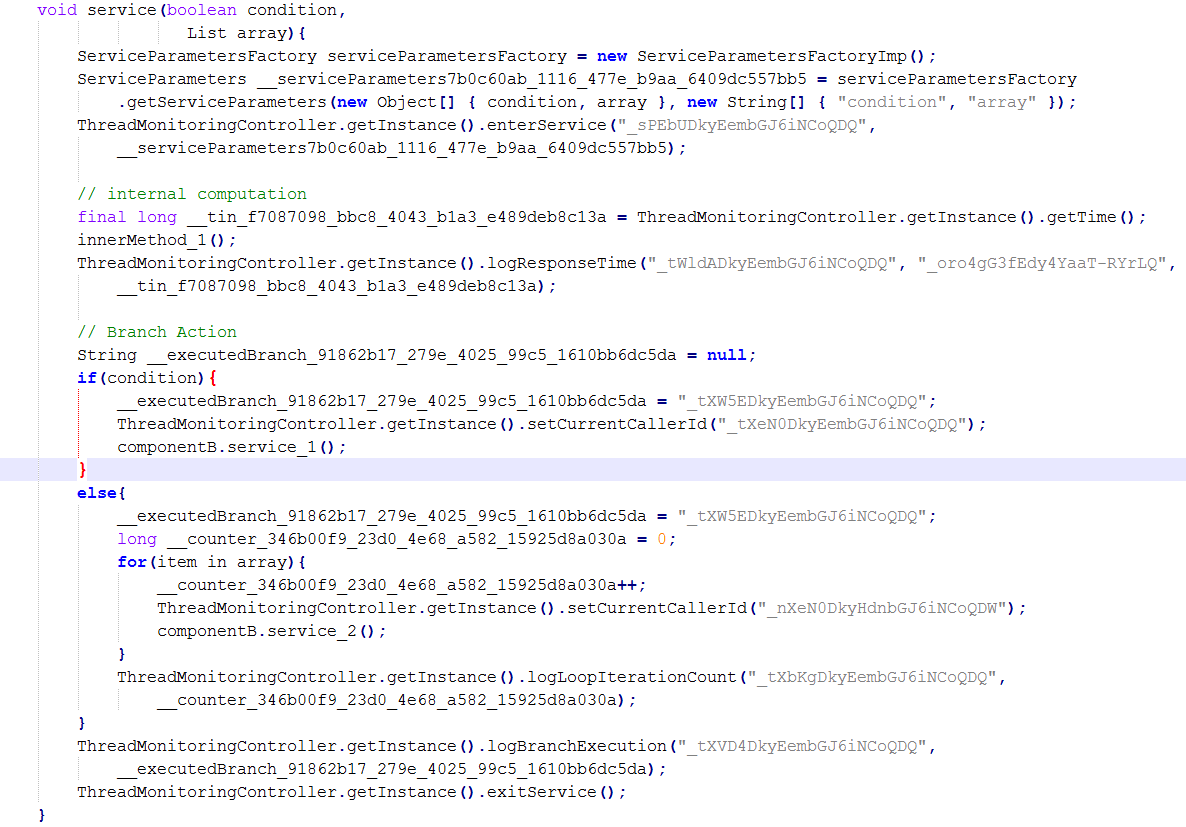
\includegraphics[width=0.9\textwidth]{figures/instrumented_code}
\caption{Instrumented version of the source code in (Figure in foundation), the instrumentation is the result of the execution of our approach}
\label{fig:instrumented_code}
\end{figure}

\section{Architecture}
\label{sec:architecture}
Figure \ref{fig:architecture} describes the architecture of our Instrumentation approach. The component diagram shows the dependencies between the components that we used to implement our approach. \\

\textbf{Two Main Concerns}\\
We distinguish between two main concerns, which are executed in diverse contexts. The first concern is related to the instrumentation of the source code. The second concern consists of the logic used to extract the services parameters and to log the monitoring information.  \\

\textbf{The Source Code Instrumentation Concern}\\
In order to instrument the source code, we provided an instrumentation process which is implemented in the component \textit{Source Code Instrumentation}. This component depends on the component \textit{Probes Provider}, which provides the fine-grained probes (Section \ref{sec:Monitoring Probes}) we defined for our instrumentation approach. The component \textit{Source Code Instrumentation} uses these probes in combination with information from the Correspondence Model(Section \ref{sec:Correspondence Meta-model})to accomplish the instrumentation of the source code. we provide more details on the instrumentation process can be found in (Section \ref{sec:Call Sequence of the Instrumentation Process}.\\


\textbf{The Monitoring Source Code Concern}\\
This concern is related to the source code that has to be executed to log the monitoring information. it can be divided into two tasks. The first one consists of the extraction of the service parameters. This task is implemented by the components \textit{Service Parameters Extractor} and \textit{Service Parameters Factory}. The first component is responsible for extracting the service parameters values and their names and pass them to the second component. The second component receives the services parameters and put them in a defined format, currently it produces a JSON file, which contains the service parameters names as the keys that their values as the values of the keys. The second task consists of the logic used to collect and log the monitoring information, which is implemented in the component \textit{Monitoring}. The component \textit{Source Code of the System} represents the source code that we want to instrument, it has dependencies to the components \textit{Monitoring} and \textit{Service Parameters Factory}.\\ 

\begin{figure}[h]
\centering
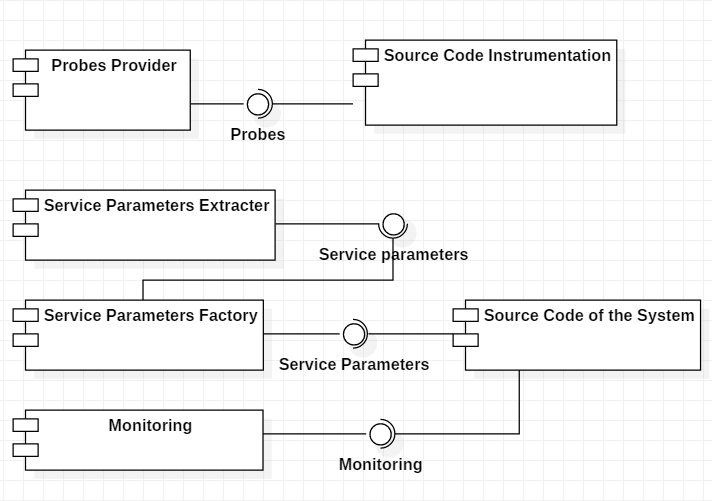
\includegraphics[width=0.9\textwidth]{figures/architecture}
\caption{The Component Diagrams shows the dependencies between the components we used to implement our approach}
\label{fig:architecture}
\end{figure}

\section{Call Sequence of the Instrumentation Process}
\label{sec:Call Sequence of the Instrumentation Process}
Figure \ref{fig:instrumentation_process} depicts the steps used in the Instrumentation Process to instrument the source code. we will describe each step in the following. \\

\textbf{Step (1): Execute the Instrumentation Process}\\
This step consists of starting the instrumentation process. Developers can execute this process at any time. Once the process is executed, it takes the probes from the Instrumentation Model (Section \ref{sec:Instrumentation Model}) and accomplish the instrumentation of the source code. \\

\textbf{Step (2): Copying the Source Code of the System}\\
Here, we create a copy of the source code, which we will instrument. As we showed in (Section \ref{sec:output}), we decided to instrument a copy of the source but not the original source code. Moreover, since we used Eclipse for our development purpose, we created a functionality that clones the original project of the system with its dependencies and properties. Therefore, the instrumentation will find place in cloned project. \\ 

\textbf{Step (4): Parse the Copied Source Code via JaMoPP}\\
In this step, we create the Java model of the source code that we want to instrument, which is the copied source code. For parsing the Java source code, we used JaMoPP (section JaMoPP). Moreover, the parsing of the source code will give us the possibility to manipulate it, like referencing the corresponding statements of a probe or the insertion of the instrumentation code in a defined position in the source code.\\

\textbf{Step (5): Returning the Monitoring Probes}\\
In this step, the Instrumentation Process calls the component Probes Provider to receive the probes that we want for the instrumentation.\\

\textbf{Step (6): Finding the Probes Statements}\\
As we mentioned before, we will instrument a copy of the source code, which means we will need find the statements in the copied source code that correspond to our probes. However, the inputs that we have for the Instrumentation Process at this stage are the probes and the corresponding statements in the original source code. That means, in order to instrument the copied source code, we will need to search the corresponding statements of the probes in the copied source code. To do this, we compared the statements of the probes in the original source code with the statements of the copied source code. \\

In order to optimize the searching for corresponding statements of the probes in the copied source code, we used three parameters to identify equal statements. The first parameter is the service in which statement is written. The second parameter is the class in which the statement find place. The third parameter is the location of the statement in the source code. The combination of these parameters is unique for every statement in the source code. Therefore, it can be used to search for the probes statements in the copied source code based on probes statements in original source code. \\

\textbf{Step (7): Instrument the Source Code}\\
In this step, the copied source code will be instrumented based on the probes and their corresponding statements that has been mapped in the previous step. Moreover, the probes are injected in the source code based on their types (section Probe).  Here, we distinguish between two kind of instrumentation, namely coarse-grained instrumentation and fine-grained instrumentation. Fine-grained instrumentation is based on the probes that are represented by the SEFF elements that we defined in (Section \ref{sec:Monitoring Probes}). Coarse-grained instrumentation consists of instrumenting the whole service without taking into account the its fine-grained probes. In this step, we execute both fine-grained and coarse-grained instrumentation. 

\textbf{Step (8): Coarse-grained Instrumentation}\\
This step consists of the coarse-grained instrumentation of all services in the source code that have been not instrumented in the previous step.  This step is required because of the adaptive instrumentation approach. As we mentioned before, in adaptive instrumentation, we collect probes only for the changed parts of the source code in the current iteration. That means, services that have been not changed in the current iteration will not be related to any probes. Thus, they will not be instrumented in the previous step. However, even tough they have been not changed in the current iteration, if they are called in the changed parts of the source code, we will need their monitoring information. Therefore, we finalized our instrumentation process by the coarse-grained instrumentation of the rest of the services of the system.  

\begin{figure}[h]
\centering
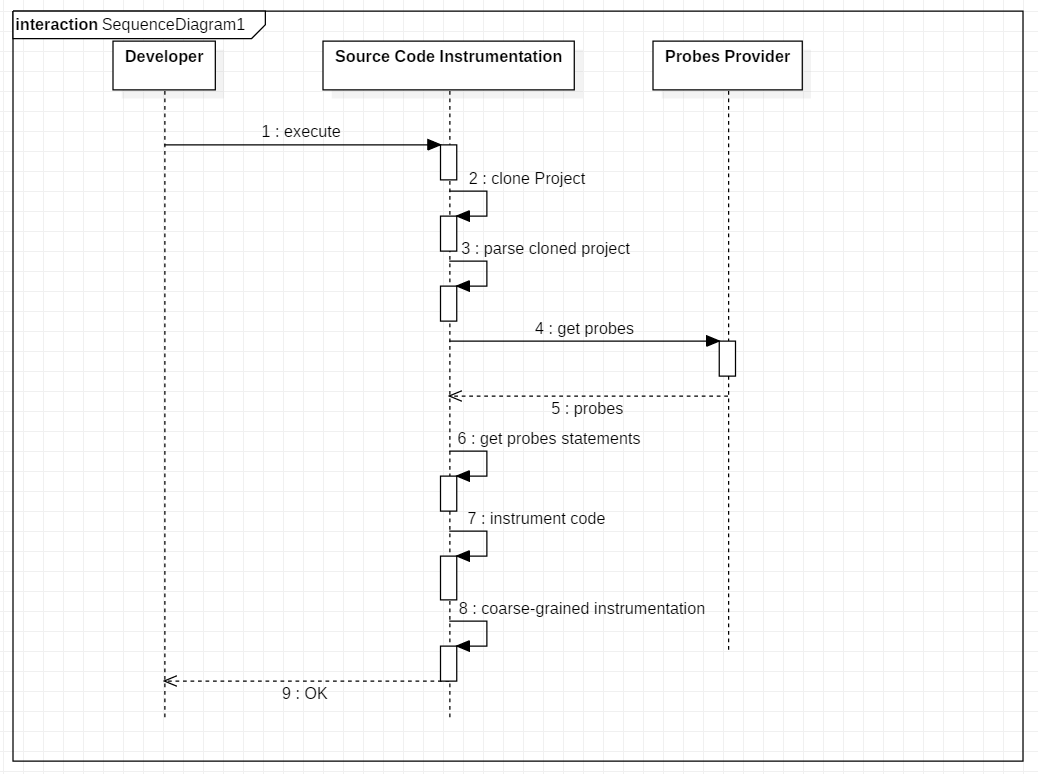
\includegraphics[width=0.9\textwidth]{figures/instrumentation_process}
\caption{Sequence Diagram that illustrates the activities of the Instrumentation Process}
\label{fig:instrumentation_process}
\end{figure}

\section{Service Parameters Extraction}
\label{sec:Service Parameters Extraction}
Manar and Koziolek showed in their approach \cite{mazkatli2018continuous} that Performance Model parameters can strongly depend on the parameters of the services. Therefore, we decided to enrich our monitoring information by extracting the service parameters and their values. \\

Figure \ref{fig:service_parameters} shows our approach for extracting the service parameters. We limited our approach to five parameter types, namely the type Map, Collection, Array, Primitive and Data Types. Data Types are the types that are defined by the user and are given as parameters to a service. For example, a DataType can be Java Bean Class named FileType, which contains the attributes file name of type string and file content of type Array of byte.\\

For service parameters extraction, we return for each parameter type only the property that has impact on the performance model. For collections and maps we extract their size. The same thing for arrays, we return their length. As for primitive types, we return the value of the parameter. Furthermore, Data types are handled via Reflection. In Data types we use reflection to search for attributes of the types Map, Collection, Array or Primitive in order to extract their defined properties. \\


\begin{figure}[h]
\centering
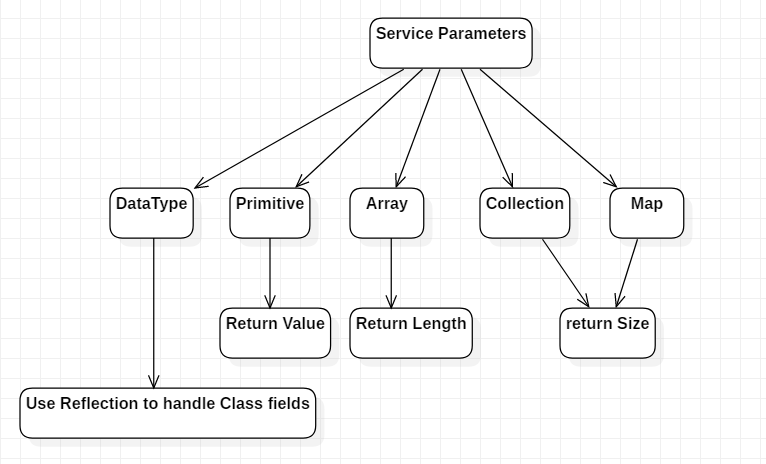
\includegraphics[width=0.9\textwidth]{figures/service_parameters}
\caption{Service parameters types and how they are extracted}
\label{fig:service_parameters}
\end{figure}


\section{Limitation}
\label{sec:Limitation}
In this section, we will present the limitation of our process for generation the monitoring probes.\\ 

\textbf{Adaptive Instrumentation is limited to Service level}\\
This limitation is due to the implementation of the SEFF Reconstruction Process (section 1.6 in  foundation) which recreates the whole SEFF of a service if a part of its source code has changed. That means, if only one element of the SEFF of the changed service has been changed, the process creates a new SEFF with new elements and replaces the old SEFF of the service. This will guide to delete the old elements of the SEFF and loose their estimated parameters, even tough they were not touched by the last changes. This limitation is reflected also on the adaptive instrumentation, the adaptive monitoring and the parameters estimation of SEFF models.\\ 

Another level that can be achieved to prevent this limitation is the statement level. In this level, only the SEFF elements that was touched by the source code changes have to be updated. In such way, we can reduce the monitoring probes which reduces the overhead of the monitoring and parameters estimation of the performance model. This can be achieved for example by comparing the SEFF of the old service and the SEFF of the new service based on the source code statements. Using this comparison, we can deduce, which element of the old SEFF has been modified, new added or deleted.  \\

\textbf{Probes with small response time must be ignored}\\
This limitation is related to service calls and internal actions. Basically, probes with response time that do not influence the performance model must be ignored. For example, an internal action that corresponds solely to a variable declaration will clearly log response time that does not affect the performance model.\\
 
We identify basically two approaches to find out if a probe with a given response time can be accepted or ignored. The First approach consists of analyzing the statements of the source code in order to decide if the probe can affect the performance model. This approach is efficient in terms of reducing the computation resources for the instrumentation, the monitoring and the parameters estimation.  However, we do not know if it's possible to apply it for all cases.\\

The second approach, which we've implemented in our approach is the filtering of the monitoring records under a defined response time value. However, this approach is applied after monitoring phase and is less efficient then the first approach because we apply the computation resources in the monitoring of probes that are not relevant. \\

If the first approach can not cover all cases, it can be used in combination with the second approach in order to improve the efficiency of the monitoring. In the first step, the first approach can be used to remove probes that has a defined number and types of statements. In the second step, the second approach will remove the records with a defined response tine value, which could not be judged by the first approach.\\


 
%% LaTeX2e class for student theses
%% sections/evaluation.tex
%% 
%% Karlsruhe Institute of Technology
%% Institute for Program Structures and Data Organization
%% Chair for Software Design and Quality (SDQ)
%%
%% Dr.-Ing. Erik Burger
%% burger@kit.edu
%%
%% Version 1.3.2, 2017-08-01

\chapter{Evaluation}
\label{ch:Evaluation}

In this section, we introduce the evaluation of our approach. We divided our evaluation into levels. In the first level, we evaluate the adaptive instrumentation. In the second level, we evaluate the monitoring information that we created to make sure that we’ve created the right monitoring information. In the third level, we evaluate our approach in term o reducing the monitoring overhead. \\
In the following we defined the goals (G) and research questions (Q) for our evaluation:\\

G1: Adaptive Instrumentation\\
  \quad Q1.1: Is our instrumentation of the source code incremental?\\
	  \qquad M1.1.1: difference between the probes in the instrumentation model and the probes logged in the        
	                monitoring information. \\
  \quad Q1.2: did we generate the right monitoring information?\\
	    \qquad M1.2.1: Number of acceptances of our monitoring information from performance model parameters  
	                         estimation approach.\\
G2: Adaptive Monitoring\\
   \hspace{10mm} Q2.1: How much monitoring overhead could we reduce?\\
        \hspace{20mm} M2.1.1: number of generated probes.\\


\section{Case Study}
\label{sec:Case Study}
In order to evaluate our approach, we performed a case study that is represented by the component diagram in Figure \ref{fig:case_study}. We created two Java interfaces and we implemented them. The first interface \textit{ISearchingAlgo} contains two functions. The service \textit{sequentianSearch}, which receives an Array of integers and a value of type integer, it returns True if the given value exists in the given array. This service is based on the sequential searching algorithm. The second service \textit{binarySearch} perform receives also an Array of integers and an integer value, it must then tell us if the given could be found in the given array. The service \textit{binarySearch} is implemented based on the binary searching algorithm. The binary searching algorithm is more efficient then the sequential searching algorithm, we choose these algorithms to provide the possibility of having different response times and service calls parameters. 

The second interface \textit{GuiSearchingAlgo} provides also two services and requires services from the interface \textit{ISearchingAlgo}. The service \textit{guiSeuentialSearch} receives two arrays of integers, the first array represents the array in which we want to perform the searching, the second array represent the values we want to search for. This service iterates over the  array of values that we want to search for and calls the service \textit{sequentialSeach} from the interface \textit{ISearchingAlgo}, which tells if the current searched value could be found. Figure 2 shows the corresponding SEFF of the \textit{guiSequentialSearch} service. The service \textit{guiBinarySearch} in the interface \textit{GuiSearchingAlgo} does the same thing as the service \textit{guiSequentialSearch} but it calls the service \textit{binarySearch} instead of \textit{sequentialSeach} service. 

\begin{figure}[h]
\centering
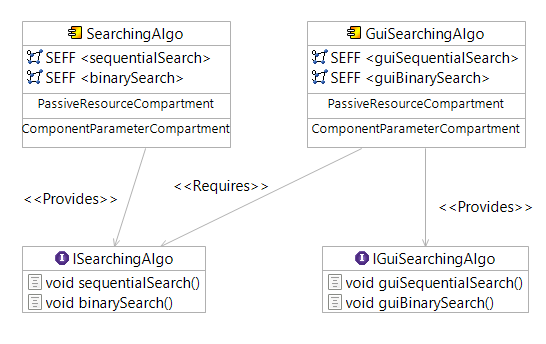
\includegraphics[width=0.9\textwidth]{figures/case_study}
\caption{Component diagram of our case study}
\label{fig:case_study}
\end{figure}




%% LaTeX2e class for student theses
%% sections/conclusion.tex
%% 
%% Karlsruhe Institute of Technology
%% Institute for Program Structures and Data Organization
%% Chair for Software Design and Quality (SDQ)
%%
%% Dr.-Ing. Erik Burger
%% burger@kit.edu
%%
%% Version 1.3.2, 2017-08-01

\chapter{Related Work}
\label{ch:Related Work}

None of the existing approaches that deal with the automatic extraction of performance
model considers the parametric dependencies of performance models, the adaptive
monitoring and the incremental execution of the whole process at the same time. Moreover,
existing approaches do not support the adaptive monitoring for performance model continuous
integration.

Walter et al. \cite{walter2017expandable} provided an expandable approach for automated extraction of
architectural performance model. He presents a framework for the extraction of
the architectural performance models based on monitoring files generalizing over
the target architectural model language. This framework can be used to create
an extraction tool for a specific modeling formalism. He implemented his approach
in so called Performance Model Extractor (PMX) tool and provided it as a web service.

Krogmann et al. \cite{krogmann2012reconstruction, krogmann2010using} used genetic programming to estimate parametric dependencies between inputs and the number of execution for each byte code instruction.
Depending on input data he could find control flow dependencies between required
and provided services. However, for receiving monitoring information, he instruments the whole system in each iteration, which causes a monitoring overhead. 

Spinner et al. \cite{spinner2016reference} predicted the system performance at run time under varying work
loads and system configuration. He proposed an approach for obtaining architectural-level model performance in virtualized environment.

Langhammer \cite{langhammer2017automated} introduced two approaches to extract the static and the dynamic
behavior of the source code. Furthermore, he proposed an approach that keeps the source code and the 
architecture consistent during development. Furthermore, he could generate the performance model incrementally. However, he did not use an adaptive monitoring approach, which means he instruments the whole system in each iteration. Therefore, the monitoring overhead could not be reduced.

Brosig et. al \cite{brosig2009automated} introduce an approach that the Palladio Component Models of of Java EE applications based on the monitoring data collected during operation. However, he did take into account the adaptive monitoring, which means he monitor the whole source code in each iteration. Therefore, monitoring huge Java EE applications will lead to monitoring overhead.    

Jägers has also introduced in his master thesis \cite{jagers2018Iterative} an approach that estimates incrementally the performance model parameters considering parametric dependencies. Moreover, he used fine-grained monitoring information for the estimation. However, he instrumented the source code manually. 

%% LaTeX2e class for student theses
%% sections/conclusion.tex
%% 
%% Karlsruhe Institute of Technology
%% Institute for Program Structures and Data Organization
%% Chair for Software Design and Quality (SDQ)
%%
%% Dr.-Ing. Erik Burger
%% burger@kit.edu
%%
%% Version 1.3.2, 2017-08-01

\chapter{Conclusions and Future Work}
\label{ch:Conclusions and Future Work}

This chapter presents a conclusion of our approach and introduces suggestions for future work. 

\subsection{Summary}
\label{sec:summary}


\subsection{Future Work}
\label{sec:future work}


%% --------------------
%% |   Bibliography   |
%% --------------------

\printbibliography


\end{document}